\documentclass[a4paper,twoside,openleft]{blocksbook}
\usepackage[cm-default]{fontspec}% provides font selecting commands
\usepackage{xunicode}% provides unicode character macros
\usepackage{xltxtra} % provides some fixes/extras
\usepackage[answerdelayed,lastexercise]{exercise}
\usepackage[labelsep=period,labelfont=it,textfont=it]{caption}
\usepackage{alltt}
\usepackage{url}
\usepackage{listings} 
\usepackage{color}
\usepackage{graphicx}
\usepackage{relsize}
\usepackage{xCJK}
\usepackage{scalefnt}
\usepackage{wrapfig}
\usepackage{everypage}
% Tables from Gnumeric.
\usepackage{array} 
\usepackage{longtable}
\usepackage{calc}
\usepackage{multirow}
\usepackage{hhline} 
\usepackage{ifthen} 
\usepackage{upquote}

\usepackage{tikz}
\usetikzlibrary{arrows,decorations.pathreplacing}
\usepackage{float}
%\usepackage{natbib}
%% Local tex stuff.
\usepackage{coderemarks}
%% Must go last.
\usepackage{hyperref}
%% special macro commands and setups for this book's style.
%% 
\setmonofont[SmallCapsFont={DejaVu Sans Mono},Scale=0.70]{DejaVu Sans Mono}
%% Fontfeatures after setting the mono font to keep
%% lstlisting fonts happy
\defaultfontfeatures{Scale=MatchLowercase,Mapping=tex-text}
\setmainfont[SmallCapsFont={Droid Sans Mono}]{Droid Serif}
\setsansfont{Droid Sans}
\def\inputGnumericTable{}

\setlength{\parindent}{0pt}
\setlength{\parskip}{0.7ex plus 0.5ex minus 0.2ex}

%%\setlength{\parskip}{0.3\baselineskip}
%%\setlength{\parindent}{0pt}
    
%% list of answers
\newlistof{listofex}{ex}{List of Exercises}
\newlistentry{exercise}{ex}{0}

\newlistof{listofcode}{code}{List of Code Examples}
\newlistentry{code}{code}{0}

%% need to do this for code examples too
%%\renewcommand{\lstlistlistingname}{List of Code Examples}
%% toc
\renewcommand{\tocheadstart}{}
\renewcommand{\aftertoctitle}{\pagestyle{blocks}}
\renewcommand{\aftertoctitle}{\thispagestyle{empty}\afterchaptertitle\pagestyle{blocks}}

%%\renewcommand{\printtoctitle}[1]{}
\renewcommand{\contentsname}{Contents}
\renewcommand{\tocmark}{\markboth{\myfamily \typename: \contentsname}{\myfamily \contentsname}}
%% new print the titles as section not as chapter, that explains
%% why the page is headerless. the page style is empty
%% lof
\renewcommand{\lofheadstart}{}
\renewcommand{\afterloftitle}{\thispagestyle{blocks}}
\renewcommand{\printloftitle}[1]{\section*{#1}}
\renewcommand{\lotmark}{\markboth{\myfamily \typename:
\contentsname}{\myfamily \listfigurename}}
%% lot
\renewcommand{\lotheadstart}{}
\renewcommand{\afterlottitle}{\thispagestyle{blocks}}
\renewcommand{\printlottitle}[1]{\section*{#1}}
\renewcommand{\lofmark}{\markboth{\myfamily \typename:
\contentsname}{\myfamily \listtablename}}
%% ex
\renewcommand{\exheadstart}{}
\renewcommand{\afterextitle}{\thispagestyle{blocks}}
\renewcommand{\printextitle}[1]{\section*{#1}}
\renewcommand{\exmark}{\markboth{\myfamily \typename: \contentsname}{\myfamily List of Exercises}}
%% code
\renewcommand{\codeheadstart}{}
\renewcommand{\aftercodetitle}{\thispagestyle{blocks}}
\renewcommand{\printcodetitle}[1]{\section*{#1}}
\renewcommand{\codemark}{\markboth{\myfamily \typename: \contentsname}{\myfamily List of Code Examples}}

\nobibintoc
\renewcommand*{\indexmark}{%
\markboth{\myfamily \typename{} \thechapter: \indexname}{\myfamily\indexname}%
}

\onecolindexfalse  %% doesn't do its things as advertised
\noindexintoc
\makeindex

%% make quote print italics and other fancy stuff
\newcommand{\qquote}{{\scalefont{4.00}{``}}}
\expandafter\def\expandafter\quote\expandafter{\quote\em}

%%\DeclareCaptionFont{white}{\color{white}}
%%\DeclareCaptionFormat{listing}{\colorbox[cmyk]{0.43, 0.35,
%%0.35,0.01}{\parbox{0.5\textwidth}{\hspace{0.5em}#1#2#3}}} % 0.98 same as listings
%%\captionsetup[lstlisting]{format=listing,labelfont=white,textfont=white,singlelinecheck=false,margin=0em,font={bf,footnotesize}}

%% Listings
\lstdefinelanguage{Go}
  {morekeywords={append,break,cap,case,chan,const,continue,copy,default,defer,else,fallthrough,%
  for,func,go,goto,if,import,interface,len,make,map,new,package,range,return,select,%
  struct,switch,type,var,%  % types
  uint8,uint16,uint32,uint64,int8,int16,int32,int64,float32,float64,byte,%
  complex,complex128,complex64,%
  int,rune,uint,bool,uintptr,string,%
  error,iota,%
  },%
  otherkeywords={<-,!,;,\{,\}},%  %% nog beter maken
    sensitive=true,%
    morecomment=[l]{//},%
    morecomment=[s]{/*}{*/},%
    morecomment=[n]{(*}{*)},%
    morestring=[b]",%
    morestring=[b]',%
    morestring=[b]`,%
  }[]%
\lstset{language=Go,inputencoding=utf8,extendedchars=false,texcl,escapechar=\|,basicstyle=\ttfamily,keywordstyle=\bfseries,numbers=none,numberblanklines=false,showstringspaces=false,breaklines=true,numberstyle=\small\ttfamily,xleftmargin=\parindent,xrightmargin=1em,linewidth=0.98\linewidth}
%,literate={"}{\textasciiquote}{1}}

\newcommand{\coderemark}[1]{\qquad$\leftarrow \textit{\small #1}$}

%% Cite style
%%\bibpunct{[}{]}{;}{s}{,}{,}

%% Exercises
\renewcommand{\ExerciseHeaderTitle}{\ExerciseTitle}
\renewcommand{\ExerciseHeaderLabel}{}
\renewcommand{\ExerciseName}{}	%% was 'Exercise'
\renewcommand{\ExerciseHeaderNB}{\theExercise}
%% This one is actually used
\renewcommand{\ExerciseHeader}{\vspace{.7ex}\noindent\textbf{Q\theExercise}. (\number\ExerciseDifficulty) \ExerciseTitle\quad%
\addcontentsline{ex}{exercise}{\numberline{\theExercise}(\number\ExerciseDifficulty) \ExerciseTitle}}
\renewcommand{\AnswerHeader}{\vspace{.7ex}\noindent\textbf{A\theExercise}.  (\number\ExerciseDifficulty) \ExerciseTitle\quad}

%% Style commands
\newcommand{\func}[1]{\texttt{#1}}
\newcommand{\key}[1]{\texttt{\textbf{#1}}}
\newcommand{\type}[1]{\texttt{\textbf{#1}}}
\newcommand{\prog}[1]{\texttt{#1}}
\newcommand{\flag}[1]{\textit{#1}}
\newcommand{\dir}[1]{\texttt{#1}}
\newcommand{\file}[1]{\texttt{#1}}
\newcommand{\var}[1]{\texttt{#1}}
\newcommand{\rem}[1]{\texttt{\textit{#1}}}
\newcommand{\package}[1]{{\textit{#1}}}
\newcommand{\first}[2]{#1\index{#2}}
\newcommand{\error}[1]{\texttt{#1}}
\newcommand{\pr}{\textbf{\%}}           %% a prompt (also bold)
\newcommand{\user}[1]{\textbf{#1}}      %% text a user should type
\newcommand{\userinput}[1]{\textit{#1}} %% text a user should choose
\newcommand{\gorelease}[1]{\texttt{#1}}

%% Footnotes
%%\renewcommand*{\thefootnote}{\textbf{\emph\MakeUppercase{\alph{footnote}}}}
\renewcommand*{\thefootnote}{\textbf{\emph\alph{footnote}}}

%% Epigraph
\newcommand{\epi}[2]{\epigraph{#1}{#2}}
\setlength{\epigraphwidth}{1.2\epigraphwidth}

%% Margin notes
\setmarginnotes{0.04\stockwidth}{0.12\stockwidth}{\onelineskip}
\newcommand{\gomarginpar}[1]{%
\marginpar{\rmfamily\itshape\small#1}}
\newcommand{\todo}[1]{%
\gomarginpar{{\textsc{TODO}}\\#1}}
%% typeset text in margin and index arg 2
\newcommand{\gomarginindex}[2]{\gomarginpar{#1}\index{#2}}
\newcommand{\gopher}{%
\begin{figure}[H]%

\includegraphics[scale=0.20, width=.70\marginparwidth]{fig/gopher.png}%
\end{figure}%
}

\newenvironment{cjk}{%
\begin{CJK*}{UTF8}{song}
\setCJKfamilyfont{Japanese}{Sazanami Gothic}
\CJKfamily{Japanese}
}%
{%
\end{CJK*}%
}
% start, end, text
\newcommand{\ubrace}[3]{%
\draw [thick,decorate,decoration={brace,amplitude=4pt},xshift=0pt,yshift=0pt] %
(#1) -- (#2) node [black,midway,below=4pt,xshift=0pt] %
{\longremark{#3}}; %
}

%% fixes
\newcommand{\exdisfix}{\vspace{1ex}}

%%%%%%%%%%%%%%%%%%%%%%%%%%%%%%%%%%%%%%%%%%%%%%%%%%%%%%%%%%%%%%%%
%% ccBeamer 0.1, 2007-07-02                                   %%
%% Written by Sebastian Pipping <webmaster@hartwork.org>      %%
%% ---------------------------------------------------------- %%
%% Licensed under Creative Commons Attribution-ShareAlike 3.0 %%
%% http://creativecommons.org/licenses/by-sa/3.0/             %%
%%%%%%%%%%%%%%%%%%%%%%%%%%%%%%%%%%%%%%%%%%%%%%%%%%%%%%%%%%%%%%%%


%% Images
\newcommand{\CcImageBy}[1]{%
	
\includegraphics[scale=#1]{creative_commons/cc_by_30.pdf}%
}
\newcommand{\CcImageCc}[1]{%
	
\includegraphics[scale=#1]{creative_commons/cc_cc_30.pdf}%
}
\newcommand{\CcImageDevNations}[1]{%
	
\includegraphics[scale=#1]{creative_commons/cc_dev_nations_30.pdf}%
}
\newcommand{\CcImageNc}[1]{%
	
\includegraphics[scale=#1]{creative_commons/cc_nc_30.pdf}%
}
\newcommand{\CcImageNd}[1]{%
	
\includegraphics[scale=#1]{creative_commons/cc_nd_30.pdf}%
}
\newcommand{\CcImagePd}[1]{%
	
\includegraphics[scale=#1]{creative_commons/cc_pd_30.pdf}%
}
\newcommand{\CcImageSa}[1]{%
	
\includegraphics[scale=#1]{creative_commons/cc_sa_30.pdf}%
}
\newcommand{\CcImageSampling}[1]{%
	
\includegraphics[scale=#1]{creative_commons/cc_sampling_30.pdf}%
}
\newcommand{\CcImageSamplingPlus}[1]{%
	
\includegraphics[scale=#1]{creative_commons/cc_sampling_plus_30.pdf}%
}


%% Groups
\newcommand{\CcGroupBy}[1]{% zoom
	\CcImageBy{#1}%
}
\newcommand{\CcGroupByNc}[2]{% zoom, gap
	\CcImageBy{#1}\hspace*{#2}\CcImageNc{#1}%
}
\newcommand{\CcGroupByNcNd}[2]{% zoom, gap
	\CcImageBy{#1}\hspace*{#2}\CcImageNc{#1}\hspace*{#2}\CcImageNd{#1}%
}
\newcommand{\CcGroupByNcSa}[2]{% zoom, gap
	\CcImageBy{#1}\hspace*{#2}\CcImageNc{#1}\hspace*{#2}\CcImageSa{#1}%
}
\newcommand{\CcGroupByNd}[2]{% zoom, gap
	\CcImageBy{#1}\hspace*{#2}\CcImageNd{#1}%
}
\newcommand{\CcGroupBySa}[2]{% zoom, gap
	\CcImageBy{#1}\hspace*{#2}\CcImageSa{#1}%
}
\newcommand{\CcGroupDevNations}[1]{% zoom
	\CcImageDevNations{#1}%
}
\newcommand{\CcGroupNcSampling}[2]{% zoom, gap
	\CcImageNc{#1}\hspace*{#2}\CcImageSampling{#1}%
}
\newcommand{\CcGroupPd}[1]{% zoom
	\CcImagePd{#1}%
}
\newcommand{\CcGroupSampling}[1]{% zoom
	\CcImageSampling{#1}%
}
\newcommand{\CcGroupSamplingPlus}[1]{% zoom
	\CcImageSamplingPlus{#1}%
}


%% Text
\newcommand{\CcLongnameBy}{Attribution}
\newcommand{\CcLongnameByNc}{Attribution-NonCommercial}
\newcommand{\CcLongnameByNcNd}{Attribution-NoDerivs}
\newcommand{\CcLongnameByNcSa}{Attribution-NonCommercial-ShareAlike}
\newcommand{\CcLongnameByNd}{Attribution-NoDerivs}
\newcommand{\CcLongnameBySa}{Attribution-ShareAlike}

\newcommand{\CcNote}[1]{% longname
	This work is licensed under the \textit{Creative Commons #1 3.0 License}.%
}


\begin{document}
\thispagestyle{empty}
\newcommand{\version}{0.5}
%% Title page
\begin{center}
\hspace{1.0cm}{\scalefont{6.00}{\sffamily{\mbox{\vspace{1.0cm}CPAM}}}}\\
\vspace{0.5cm}
{\scalefont{3.0}\sffamily{Cross-Platform Application Management}}
\end{center}
\vspace*{2cm}
\begin{figure}[h!]
\begin{center}
    
\includegraphics[scale=0.65]{fig/bumper-inverse.png}
\end{center}
\end{figure}
\vspace*{0.02\stockheight}
\begin{minipage}{0.4\textwidth}
\begin{flushleft} \large
\hspace*{2,0cm}Author:\\
\hspace*{2.0cm}\emph{T.J. Yang}\\
\vfill
\end{flushleft}
\end{minipage}
\hspace{5mm}
\begin{minipage}{0.4\textwidth}
\begin{flushright} \large
Thanks to:\\
\emph{TWW Inc.} \\
\vfill
\end{flushright}
\end{minipage}
\vspace*{0.5cm}
\begin{center}
With the help and contributions from: 

({\small in alphabetical order})

\emph{Anthony Magro},
\emph{Uriel}.

\end{center}
\vfill
\begin{center}
    \hspace*{1cm}\CcGroupByNcSa{0.83}{0.95ex}\\[2.5ex]
    \hspace*{1cm}{\tiny\CcNote{\CcLongnameByNcSa}}
\end{center}
\begin{center}
\hspace*{1cm}\emph{T.J. Yang -- \copyright 2012 - 2013}
\end{center}
\vspace{-3em}
%% End title page %%

\newpage

\thispagestyle{empty}
\begin{figure}[H]
\begin{center}
\emph{
This work is licensed under the Attribution-NonCommercial-ShareAlike 3.0 Unported License. To
view a copy of this license, visit \url{http://creativecommons.org/licenses/by-nc-sa/3.0/} 
or send a letter
to Creative Commons, 171 Second Street, Suite 300, San Francisco, California, 94105, USA.}
\vspace{2em}

\emph{All example code used in this book is hereby put in the public domain.}
%%PDFcrop fails on Ubuntu
%%\includegraphics[scale=0.50]{fig/google_logo_black.pdf}
\end{center}
\end{figure}
\begin{center}
\vfill
\emph{Extension of TWW Inc. toolsets to open source OS}
(\emph{\version})

\tiny{Software Pacakge creation and management across OS platform made easy}
\vspace{.2\stockheight}
\end{center}

\clearpage

\pagenumbering{roman}
\tableofcontents*
\listoffigures*
%%\listoftables* %% there are so few
\listofcode* 
\listofex* 
\clearpage

\chapter*{Preface}
\label{chap:preface}
\epi{``Is Go an object-oriented language? Yes and no.''}
{\textit{Frequently asked questions}\\ \textsc{GO AUTHORS}}

\section*{Audience}
\noindent{}This is an introduction to the Go language from Google. Its aim
is to provide a guide to this new and innovative language. 

The intended audience of this book is people who are familiar with programming
and know some programming languages, be it C\cite{c}, C++\cite{c++}, 
Perl\cite{perl}, Java\cite{java}, Erlang\cite{erlang}, Scala\cite{scala} or
Haskell\cite{haskell}. This is \emph{not} a book which teaches you how to 
program, this is a book that just teaches you how to use Go.

As with
learning new things, probably the best way to do this is to discover it for
yourself by creating your own programs.
Each chapter therefore includes a number of exercises (and answers)
to acquaint you with the language.
An exercise
is numbered as \textbf{Q$n$}, where $n$ is a number. After the
exercise number another number in parentheses displays the difficulty
of this particular assignment. This difficulty ranges from 0 to
9, where 0 is easy and 9 is difficult. 
Then a short name is given, for easier reference.
For example:
\begin{verse}
\textbf{Q1}. (1) A map function \ldots
\end{verse}
introduces a question numbered \textbf{Q1} of a level 1 difficulty, concerning a
\func{map()}-function. The answers are included after the exercises on a
new page.
The numbering and setup of the answers is identical to the
exercises, except that an answer starts with \textbf{A$n$}, where the
number $n$ corresponds with the number of the exercise. Some exercises
don't have an answer, they are marked with an asterisks.

\section*{Book layout}
\begin{description}
\item[Chapter \ref{chap:intro}: \titleref{chap:intro}]
A short introduction and history of Go. It
tells how to get the source code of Go itself. It assumes a Unix-like environment, although
Go should be fully usable on Windows.

\item[Chapter \ref{chap:basics}: \titleref{chap:basics}] 
Tells about the basic types, variables and control
structures available in the language.

\item[Chapter \ref{chap:functions}: \titleref{chap:functions}] 
In the third chapter we look at functions, the basic building blocks of Go programs.

\item[Chapter \ref{chap:packages}: \titleref{chap:packages}] 
In chapter \ref{chap:packages} we see that functions and data can be grouped together
in packages. You will also see how to document and test your packages.

\item[Chapter \ref{chap:beyond}: \titleref{chap:beyond}] 
After that we look at creating your own types in chapter \ref{chap:beyond}. It also
looks at allocation in Go.

\item[Chapter \ref{chap:interfaces}: \titleref{chap:interfaces}] 
Go does not support Object Orientation in the traditional sense.
In Go the central concept is interfaces.

\item[Chapter \ref{chap:channels}: \titleref{chap:channels}] 
With the \func{go} keyword functions can be started in separate routines (called goroutines). 
Communication with those goroutines is done via channels. 

\item[Chapter \ref{chap:communication}: \titleref{chap:communication}] 
In the last chapter we show how to interface with the rest of the world from within 
a Go program. How create files and read and wrote from and to them. We also briefly
look into networking.
\end{description}

I hope you will enjoy this book and the language Go.

\section*{Settings used in this book}
\begin{itemize}
\item Go itself is installed in \file{\~{}/go} ;
\item Go source code we want to compile ourself is placed in \file{\~{}/g/src} and
\var{\$GOPATH} is set to \var{GOPATH=\~{}/g} .
\end{itemize}

\begin{flushright}
Miek Gieben, 2011, 2012 -- \url{miek@miek.nl}
\end{flushright}


\chapter{Introduction}
\pagenumbering{arabic}
\label{chap:intro}
\epi{``I am interested in this and hope to do something.''}
{\textit{On adding complex numbers to Go}\\ \textsc{KEN THOMPSON}}

\noindent{}What is Go? From the website \cite{go_web}:
\begin{quote}
The Go programming language is an open source project to make
programmers more productive. Go is expressive, concise, clean, and
efficient. Its concurrency mechanisms make it easy to write programs
that get the most out of multi core and networked machines, while its
novel type system enables flexible and modular program construction. Go
compiles quickly to machine code yet has the convenience of garbage
collection and the power of run-time reflection. It's a fast, statically
typed, compiled language that feels like a dynamically typed,
interpreted language.
\end{quote}

Go is a young language, where 
features are still being added or even \emph{removed}. It 
may be possible that some text is outdated when you
read it. 
Some exercise answers may become incorrect as Go continues
to evolve.
We will do our best to keep this document up to 
date with respect to the latest Go release.
An effort has been made to create ``future proof'' code examples.

The following convention is used throughout this book:
\begin{itemize}
\item Code is displayed in \prog{DejaVu Mono};
\item Keywords are displayed in \key{DejaVu Mono Bold};
\item Comments are displayed in \rem{DejaVu Mono Italic};
\item Extra remarks in the code \coderemark{Are displayed like this};
\item Longer remarks get a number -- \gocircle{1} -- with the explanation following;
\item Line numbers are printed on the right side;
\item Shell examples use a \pr{} as prompt;
\item User entered text in shell examples \texttt{\user{is in bold}}, system responses
are in a \texttt{typewriter font};
\item An emphasized paragraph is indented and has a vertical bar on the
left.
\end{itemize}

\section{Official documentation}
There already is a substantial amount of documentation written about Go.
\gomarginpar{When searching on the internet use the term ``golang'' instead of plain ``go''.}
The Go Tutorial \cite{go_tutorial}, and the Effective Go
document \cite{effective_go}. The
website \url{http://golang.org/doc/} is a very good starting point
for reading up on Go\footnote{\url{http://golang.org/doc/} itself is served by 
a Go program called \prog{go\ doc}.}. Reading these documents is
certainly not required, but is recommended.

Go comes with its own documentation in the form of a program called
\prog{go doc}. 
You can use it yourself to look
in the on-line documentation. For
instance, suppose we want to know more about the package \package{hash}.
We would then give the command \prog{go doc hash}.
How to create your own package documentation
is explained in chapter \ref{chap:packages}.

\section{Origins}
Go has it origins in Inferno \cite{inferno} (which in turn was based
upon Plan 9 \cite{plan9}). Inferno included a language called Limbo
\cite{limbo}. Quoting from the Limbo paper:
\begin{quote}
Limbo is a programming language intended for applications running
distributed systems on small computers. It supports modular programming,
strong type checking at compile- and run-time, \emph{inter process
communication over typed channels}, automatic \emph{garbage collection}, and
simple abstract data types. It is designed for safe execution even on
small machines without hardware memory protection.
\end{quote}
A feature Go inherited from Limbo is channels (see chapter
\ref{chap:channels}). Again from the Limbo documentation.
\begin{quote}
[A channel] is a communication mechanism capable of sending and receiving objects of
the specified type to another agent in the system. Channels may be used
to communicate between local processes; using library procedures, they
may be connected to named destinations. In either case send and receive
operations may be directed to them.
\end{quote}
The channels in Go are easier to use than those in Limbo.
If we dig even deeper in the history of Go we also find references
to ``Newsqueak'' \cite{newsqueak}, which pioneered the use of 
channel communication in a C--like language. Channel
communication isn't unique to these languages, a big non--C--like
language which also uses them is Erlang \cite{erlang}.

\begin{figure}[H]
\caption{Chronology of Go}
\label{fig:chrono-of-go}
\begin{center}
\includegraphics[scale=0.65]{fig/go-history.pdf}
\end{center}
\end{figure}

The whole of idea of using channels to communicate with other processes
is called Communicating Sequential Processes (CSP) and was conceived
by C. A. R. Hoare \cite{hoare}, who incidentally is the same man that
invented QuickSort \cite{quicksort}.

\begin{lbar}[]
Go is the first C--like language that is widely available,
runs on many
different platforms and makes concurrency easy (or easier).
\end{lbar}

\section{Getting Go}
In this section we tell how to install Go locally on your machine, but you can
also compile Go code online at \url{http://play.golang.org/}. To quickly
play with code this is by far the easiest route.

Ubuntu and Debian both have a Go package in their repositories, look for
the package ``golang''. But there are still some minor issues being worked
out. For now we will stick to the installation from source.

So we will retrieve the code from the mercurial archive and compile
Go yourself. For other Unix like systems the procedure is the same.
\begin{itemize}
\item First install Mercurial (to get the \prog{hg} command). In
Ubuntu/Debian/Fedora you must install the \prog{mercurial} package;

\item For building Go you need the packages: \prog{bison},
\prog{gcc}, \prog{libc6-dev}, \prog{ed}, \prog{gawk} and \prog{make};

\item Set the environment variable \prog{GOROOT} to the root of your
Go install:
\begin{display}
\pr \user{export GOROOT=/go}
\end{display}

\item Then retrieve the Go source code:
\begin{display}
\pr \user{hg clone -r release https://go.googlecode.com/hg/ $GOROOT}
\end{display}

\item Set your PATH to so that the Shell can find the Go binaries:
\begin{display}
\pr \user{export PATH=$GOROOT/bin:$PATH}
\end{display}
\item Compile Go
\begin{display}
\pr \user{cd $GOROOT/src}
\pr \user{./all.bash}
\end{display}
\end{itemize}
If all goes well, you should see the following at the end:
\begin{display}
--- cd ../test
0 known bugs; 0 unexpected bugs

ALL TESTS PASSED

---
Installed Go for linux/amd64 in /home/go
Installed commands in /home/go/bin
\end{display}
You now have Go installed on your system and you can start playing.
Note that currently (March 2012) this install version r60 of, this version
is old. If you want Go1, or something close to it, you will have to
upgrade to the latest weekly, see the section ``\titleref{sec:weekly}''.


\section{Keeping up to date}
\label{sec:weekly}
New releases are announced on the Go Nuts mailing list \cite{go_nuts}. To update an
existing tree to the latest release, you can run:
\begin{display}
\pr \user{cd $GOROOT}
\pr \user{hg pull}
\pr \user{hg update release}
\pr \user{cd src}
\pr \user{./all.bash}
\end{display}
\noindent{}To see what you are running right now:
\begin{display}
\pr \user{cd $GOROOT}
\pr \user{hg identify}
79997f0e5823 release/release.2010-10-20
\end{display}
\noindent{}That would be release \gorelease{2010-10-20}. The release as 
describe is a ``stable'' releases,
as opposed to the ``weekly'' releases that are more volatile. 
If you want to track the weekly releases
instead of the stable ones you can use:
\begin{display}
\pr \user{hg update weekly}
\end{display}
In stead of
\begin{display}
\pr \user{hg update release}
\end{display}

\section{Exercises}
\begin{Exercise}[title={Documentation},difficulty=1]
\label{ex:doc}
\Question
Go's documentation can be read with the \prog{go doc} program, which is
included the Go distribution.

\prog{go doc hash} gives information about the \package{hash} package. Reading the
documentation on \package{compress} gives the following result:
\vskip\baselineskip
\begin{display}
\pr \user{go doc compress}
SUBDIRECTORIES

        bzip2
        flate
        gzip
        lzw
        testdata
        zlib
\end{display}
\vskip\baselineskip
With which \prog{go doc} command can you read the documentation of \package{gzip} contained in
\package{compress}?

\end{Exercise}

\begin{Answer}
\Question
The package \package{gzip} is in a \emph{subdirectory} of
\package{compress}, so you will only need\quad \texttt{go doc compress/gzip}.

Specific functions inside the ``Go manual'' can also be accessed. For
instance the function \func{Printf} is described in \package{fmt}, but to
only view the documentation concerning this function use: \prog{go doc fmt Printf}{} .

You can even display the source code with: \prog{go doc -src fmt Printf} .     

All the built-in functions are also accesible by using go doc: \prog{go doc builtin}.
\end{Answer}


\cleardoublepage
\section{Answers}
\shipoutAnswer


\chapter{Basics}
\label{chap:basics}

\epi{"In Go, the code does exactly what it says on the page."}{\textit{Go
Nuts mailing list}\\\textsc{ANDREW GERRAND}}

\noindent{} There are three main components to make a package management system.

\begin{description}
\item[Software Build]
This component has tools for us to build software from source code in the form tar ball or source tree on source code management system.
\item[Software Package Creation]

\item[Package Distribution] 
Communication with these goroutines is done
via \first{channels}{channels} \cite{csp, hoare};

\end{description}

Erlang \cite{erlang} also shares some
of the features of Go. Notable differences between Erlang
and Go is that Erlang borders on being a functional language,
where Go is an imperative one. And Erlang runs in a virtual
machine, while Go is compiled. Go also has a much more Unix-like
feeling to it.

\section{Hello World}
\label{sec:hello world}
In the Go tutorial, Go is presented to the world in the typical
manner: letting it print "Hello World" (Ken Thompson and
Dennis Ritchie started this when they presented the C language in 
the nineteen seventies). We don't think we can do better, so 
here it is, ''Hello World'' in Go.

\lstinputlisting[numbers=right,label=src:hello,caption=Hello world]{src/helloworld.go}
Lets look at the program line by line.
\showremarks

\section{Compiling and running code}
\label{sec:building a program}
The preferred way to build a Go program, is to use a
the \prog{go} tool.\index{tooling!go}

To build \prog{helloworld} we just give:
\begin{display}
\pr \user{go build helloworld.go}
\end{display}
\index{tooling!go!build}
This results in a executable called \prog{helloworld}.

\begin{display}
\pr \user{./helloworld}
\end{display}
\vspace{-3.0ex}
\texttt{Hello, world; or }%
\begin{math}\kappa\alpha\lambda\eta\mu\acute{\epsilon}\rho\alpha\hspace{1em}\kappa\end{math}%
\'o\begin{math} \sigma\mu\epsilon\end{math}\texttt{; or }\begin{cjk}こんにちは 世界\end{cjk}
\ \newline
\ \newline

\section{Settings used in this book}
\label{sec:settings used}
\begin{itemize}                            
\item Go itself is installed in \file{\~{}/go} ;                     
\item Go source code we want to compile ourself is placed in \file{\~{}/g/src} and
\var{\$GOPATH} is set to \var{GOPATH=\~{}/g} . This variable comes into play
when start using packages (chapter \ref{chap:packages}).
\end{itemize}

\section{Variables, types and keywords}
\label{sec:vars}
In the next sections we will look at variables, basic types,
keywords and control structures of our new language. 
Go has a C-like feel when it comes to its syntax. 
If you want to put two (or more) statements on one line, they must be
separated with a semicolon (';'). Normally you don't need the semicolon.

Go is different from other languages in that the type of a variable
is specified \emph{after} the variable name. So not: 
\lstinline{int a}, but \lstinline{a int}. When declaring a variable it
is assigned the "natural" null value for the type. This means that after
\lstinline{var a int}, \lstinline{a} has a value of 0. With
\lstinline{var s string}, \lstinline{s} is assigned the zero string,
which is \lstinline{""}. 

Declaring and assigning in Go is a two step process, but they may
be combined. Compare the following pieces of code which have
the same effect. 
\index{variables!declaring}
\index{variables!assigning}

\begin{minipage}{.5\textwidth}
\begin{lstlisting}[linewidth=.5\textwidth,caption={Declaration with =}]
var a int
var b bool
a = 15
b = false
\end{lstlisting}
\hfill
\end{minipage}
\begin{minipage}{.5\textwidth}
\begin{lstlisting}[linewidth=.5\textwidth,caption={Declaration with :=}]
a := 15
b := false
\end{lstlisting}
\ \\
\ \\
\hfill
\end{minipage}

On the left we use the
\key{var} keyword to declare a variable and \emph{then} assign a value to
it. The code on the right uses \mbox{\key{:=}{ }} to do this in one
step (this form may only be used \emph{inside} functions).
In that case the variable
type is \emph{deduced} from the value. A value of 15 indicates an \type{int},
a value of \texttt{false} tells Go that the type should be \type{bool}. 
Multiple \key{var} declarations may also be grouped, \key{const}
and \key{import} also allow this. Note the use of parentheses:
\begin{lstlisting}
var (
    x int
    b bool
)
\end{lstlisting}
Multiple variables of the same type can also be declared on a
single line: \lstinline{var x, y int}, makes \var{x} and \var{y} both
\type{int} variables. You can also make use of \first{parallel
assignment}{parallel assignment}:
\begin{lstlisting}
a, b := 20, 16
\end{lstlisting}
Which makes \var{a} and \var{b} both integer variables and assigns
20 to \var{a} and 16 to \var{b}.

A special name for a variable is \var{\textbf{\_}} \index{variables!\_}
(underscore) \index{variables!underscore}. Any value
assigned to it is discarded. In this example we only assign the integer
value of 35 to \var{b} and discard the value 34.
\begin{lstlisting}
_, b := 34, 35
\end{lstlisting}
Declared, but otherwise unused variables are a compiler error in Go. The
following code generates this error:
\error{i declared and not used}

\begin{lstlisting}
package main
func main() { 
    var i int
}
\end{lstlisting}

\subsection{Boolean types}
A boolean type represents the set of boolean truth values denoted by the
predeclared constants \emph{true} and \emph{false}. The boolean type is \type{bool}.

\subsection{Numerical types}
Go has the well known types such as \lstinline{int}, this type
has the appropriate length for your machine. 
Meaning that on a 32 bits machine they are 32 bits, and on
a 64 bits machine they are 64 bits. Note: an \lstinline{int} is
either 32 or 64 bits, no other values are defined. Same goes 
for \lstinline{uint}.

If you want to be explicit about the length you can have
that too with \lstinline{int32}, or \lstinline{uint32}. The full
list for (signed and unsigned) integers is
\type{int8}, \type{int16}, \type{int32}, \type{int64} and
\type{byte}, \type{uint8}, \type{uint16}, \type{uint32}, \type{uint64}.
With \lstinline{byte} being an
alias for \lstinline{uint8}. For floating point values there is
\lstinline{float32} and \lstinline{float64} (there is no \lstinline{float} type). 
A 64 bit integer or floating point value is \emph{always} 64 bit, also on 32 bit
architectures.

Note however
that these types are all distinct and assigning variables which mix
these types is a compiler error, like in the following code:
\lstinputlisting[numbers=right,label=src:types,caption=Familiar types are still distinct]{src/types.go}
Gives the error on the assignment on line 7:

\noindent\error{types.go:7: cannot use a + a (type int)  as type int32 in assignment}

The assigned values may be denoted using octal, hexadecimal or the scientific notation:
\lstinline{077}, \lstinline{0xFF}, \lstinline{1e3} or
\mbox{\lstinline{6.022e23}} are all valid.

\subsection{Constants}
\label{sec:constants}
Constants in Go are just that --- constant. They are created at compile
time, and can only be numbers, strings or booleans;
\lstinline{const x = 42} makes \var{x} a constant. You can use
\first{\key{iota}}{keyword!iota} \footnote{The word [iota] is used in a common English phrase,
'not one iota', meaning 'not the slightest difference', in reference to
a phrase in the New Testament: ``\emph{until heaven and earth pass away, not an
iota, not a dot, will pass from the Law}.'' \cite{iota}}
to enumerate values.
\begin{lstlisting}
const (
	a = iota
	b = iota 
)
\end{lstlisting}
The first use of \key{iota} will yield 0, so \var{a} is equal to 0, whenever
\key{iota} is used again on a new line its value is incremented with 1, so \var{b}
has a value of 1.

You can even do the following, let Go repeat the use of \key{= iota}:
\begin{lstlisting}
const (
	a = iota
	b	    |\coderemark{Implicitly \texttt{b = iota}}|
)
\end{lstlisting}
You may also explicitly type a constant, if you need that:
\begin{lstlisting}
const (
	a = 0           |\coderemark{Is an \key{int} now}|
	b string = "0" 
)
\end{lstlisting}

\subsection{Strings}
An important other built in type is \lstinline{string}. Assigning a
string is as simple as:
\begin{lstlisting}
s := "Hello World!"
\end{lstlisting}
Strings in Go are a sequence of UTF-8 characters enclosed in double
quotes ("). If you use the single quote (') you mean one character
(encoded in UTF-8) --- which is \emph{not} a \lstinline{string} in Go.

Once assigned to a variable the string can not be changed anymore: strings in Go are
immutable. For
people coming from C, the following is not legal in Go:
\begin{lstlisting}
var s string = "hello"
s[0] = 'c'  |\coderemark{Change first char. to 'c', this is an error}|
\end{lstlisting}
To do this in Go you will need the following:
\begin{lstlisting}
s := "hello"
c := []byte(s)	    |\longremark{Convert \var{s} to an array of bytes, see %
chapter \ref{chap:beyond} section "\titleref{sec:conversions}" on %
page \pageref{sec:conversions};}|
c[0] = 'c'	    |\longremark{Change the first element of this %
array;}|
s2 := string(c)     |\longremark{Create a \emph{new} %
string \var{s2} with the alteration;}|
fmt.Printf("%s\n", s2) |\longremark{print the string with \func{fmt.Printf}.}|
\end{lstlisting}
\showremarks

\begin{lbar}[Multi-line strings]
Due to the insertion of semicolons (see \cite{effective_go} section
``Semicolons''), you need to be careful with using multi line strings. If
you write:
\begin{lstlisting}
s := "Starting part"
    + "Ending part"
\end{lstlisting}
This is transformed into:
\begin{lstlisting}
s := "Starting part";
    + "Ending part";
\end{lstlisting}
Which is not valid syntax, you need to write:
\begin{lstlisting}
s := "Starting part" +
     "Ending part"
\end{lstlisting}
Then Go will not insert the semicolons in the wrong places. Another way
would be to use \emph{raw} string literals\index{string literal!raw} by using back quotes: \key{`}:
\begin{lstlisting}
s := `Starting part
     Ending part`
\end{lstlisting}
Be aware that in this last example \var{s} now also contains the newline.
Unlike \emph{interpreted} string literals \index{string literal!interpreted} a raw string literal's value
is composed of the \emph{uninterpreted} characters between the quotes.
\end{lbar}

\subsection{Runes}
\lstinline{Rune} is an alias for int. 

\subsection{Complex numbers}
Go has native support for complex numbers. If you 
use them you need a variable of the type \lstinline{complex128} (64
bit imaginary part). If you
want something smaller there is \lstinline{complex64} -- for a 32 bits
imaginary part.
Complex numbers are written as
\var{re + im$i$}, where \var{re} is the real part,
\var{im} is the imaginary part and $i$ is the literal '$i$' ($\sqrt{-1}$).
An example of using complex numbers:

\lstinline{var c complex64 = 5+5i; fmt.Printf("Value is: %v", c)}\newline
will print: \lstinline{(5+5i)}

\subsection{Errors}
Any non-trivial program will have the need for error reporting sooner or later. Because of this
Go has a builtin type specially for errors, called \lstinline{error}.

\section{Operators and built-in functions}
Go supports the normal set of numerical operations,
table \ref{tab:op-precedence}
lists the current ones and their relative precedence. They
all associate from left to right.

\begin{table}[H]
\begin{center}
\caption{Operator precedence}
\label{tab:op-precedence}
\begin{tabular}{ll}
%%\toprule
\textbf{Precedence} & \textbf{Operator(s)} \\ \midrule
Highest   &	\verb!*  /  %  <<  >>  &  &^!		\\
    &	\verb!+  -  | ^!			\\
    &	\verb+==  !=  <  <=  >  >=+		\\
    &	\verb!<-!				\\
    &	\verb!&&!				\\
Lowest    &	\verb!||!				\\
%%\bottomrule
\end{tabular}

\end{center}
\end{table}
\verb|+ - * /| and \verb|%| all do what you would expect,
\verb!& | ^!
and \verb!&^! are bit operators for
\first{bitwise and}{operator!bitwise!and}, 
\first{bitwise or}{operator!bitwise!or}, \first{bitwise xor}{operator!bit
wise xor} and \first{bit clear}{operator!bitwise!clear} respectively.
The \verb|&&| and \verb/||/ operators are 
logical \first{and}{operator!and} and
logical \first{or}{operator!or}. Not listed in the table
is the logical \first{not}{operator!not}: \verb/!/

Although Go does not support operator overloading (or method
overloading for that matter), some of the built-in
operators \emph{are} overloaded. For instance \texttt{+} can be used for integers,
floats, complex numbers and strings (adding strings is concatenating
them). 

\section{Go keywords}
\begin{table}[H]
\begin{center}
\caption{Keywords in Go}
\label{tab:keywords}
%%%%%%%%%%%%%%%%%%%%%%%%%%%%%%%%%%%%%%%%%%%%%%%%%%%%%%%%%%%%%%%%%%%%%%
%%                                                                  %%
%%  This is a LaTeX2e table fragment exported from Gnumeric.        %%
%%                                                                  %%
%%%%%%%%%%%%%%%%%%%%%%%%%%%%%%%%%%%%%%%%%%%%%%%%%%%%%%%%%%%%%%%%%%%%%%
\begin{tabular}{lllll}
\key{break}	&\key{default}	&\key{func}	&\key{interface} &\key{select}\\
\key{case}	&\key{defer}	&\key{go}	&\key{map} &\key{struct}\\
\key{chan}	&\key{else}	&\key{goto}	&\key{package} &\key{switch}\\
\key{const}	&\key{fallthrough}	&\key{if}	&\key{range} &\key{type}\\
\key{continue}	&\key{for}	&\key{import}	&\key{return} &\key{var}\\
\end{tabular}

\end{center}
\end{table}
Table \ref{tab:keywords} lists all the keywords in Go. 
In the following paragraphs and chapters we will cover them. Some
of these we have seen already.
\begin{itemize}
\item For \key{var} and \key{const} see section ``\titleref{sec:vars}'' on 
page \pageref{sec:vars};
\item \key{package} and \key{import} are briefly touched upon in section ``\titleref{sec:hello world}''. 
In chapter \ref{chap:packages} they are documented in more detail.
\end{itemize}
Others deserve more text and have their own chapter/section:
\begin{itemize}
\item \key{func} is used to declare functions and methods;
\item \key{return} is used to return from functions, for both \key{func}
and \key{return} see chapter \ref{chap:functions} for the details;
\item \key{go} is used for concurrency (chapter \ref{chap:channels});
\item \key{select} used to choose from different types of communication, see chapter \ref{chap:channels};
\item \key{interface} see chapter \ref{chap:interfaces};
\item \key{struct} is used for abstract data types, see chapter \ref{chap:beyond};
\item \key{type} also see chapter \ref{chap:beyond}.
\end{itemize}

\section{Control structures}
There are only a few control structures in 
Go \footnote{This section is copied from \cite{effective_go}.}.
For instance there is no do or while loop, only a 
\key{for}. There is a (flexible) \key{switch} statement and \key{if} and
\key{switch} accept an
optional initialization statement like that of \key{for}. There also is
something called a type switch and a multiway communications
multiplexer, \key{select} (see chapter \ref{chap:channels}). The syntax is 
different (from that in C): parentheses
are not required and the body must \emph{always} be brace-delimited.

\subsection{If-else}
In Go an \first{\key{if}}{keyword!if} looks like this:
\begin{lstlisting}
if x > 0 {	|\coderemark{\{ is mandatory}|
    return y
} else {
    return x
}
\end{lstlisting}
Mandatory braces encourage writing simple \key{if} statements on multiple
lines. It is good style to do so anyway, especially when the body
contains a control statement such as a
\first{\key{return}}{keyword!return} or
\first{\key{break}}{keyword!break}.

Since \key{if} and \key{switch} accept an initialization statement, it's common to
see one used to set up a (local) variable.
\begin{lstlisting}
if err := file.Chmod(0664); err != nil {  |\coderemark{\texttt{nil} is %
like C's NULL}|
    log.Stderr(err) |\coderemark{Scope of \var{err} is limited to %
\key{if}'s body}|
    return err
}
\end{lstlisting}
You can use the logical operators (see table \ref{tab:op-precedence}) as
you would normally do:
\begin{lstlisting}
if true && true  {
    println("true")
}
if ! false {
    println("true")
}
\end{lstlisting}

In the Go libraries, you will find that when an \key{if} statement doesn't flow
into the next statement -- that is, the body ends in \key{break},
\key{continue}, \key{goto},
or \key{return} -- the unnecessary \first{\key{else}}{keyword!else} is omitted.

\begin{lstlisting}
f, err := os.Open(name, os.O_RDONLY, 0)
if err != nil {
    return err
}
doSomething(f)
\end{lstlisting}
This is a example of a common situation where code must analyze a
sequence of error possibilities. The code reads well if the successful
flow of control runs down the page, eliminating error cases as they
arise. Since error cases tend to end in \key{return} statements, the resulting
code needs no \key{else} statements.
\begin{lstlisting}
f, err := os.Open(name, os.O_RDONLY, 0)
if err != nil {
    return err
}
d, err := f.Stat()
if err != nil {
    return err
}
doSomething(f, d)
\end{lstlisting}
Syntax wise the following is illegal in Go:
\begin{lstlisting}
if err != nil
{		    |\coderemark{Must be on the same line as the if}|
    return err
}
\end{lstlisting}
See \cite{effective_go} section ``Semicolons'' for the deeper reasons
behind this.

\begin{lbar}[Ending with \key{if-then-else}]
Note that if you end a function like this:
\begin{lstlisting}
if err != nil {
    return err
} else {
    return nil
}
\end{lstlisting}
It will not compile. This is a bug in the Go compiler. See
\cite{go_issue_65} for an extended problem description and
hopefully a fix.
\end{lbar}

\subsection{Goto}
Go has a \first{\key{goto}}{keyword!goto} statement --- use it wisely. With \key{goto}
you jump to a \index{label} label which must be defined within the current function.
For instance a loop in disguise:
\begin{lstlisting}
func myfunc() {
        i := 0                                                                                      
Here:	   |\coderemark{First word on a line ending with a colon is a label}|
        println(i)
        i++ 
        goto Here |\coderemark{Jump}|
}
\end{lstlisting}
The name of the label is case sensitive.

\subsection{For}
\label{sec:for}
The Go \first{\key{for}}{keyword!for} loop has three forms, only one of
which has semicolons.
\begin{lstlisting}
for init; condition; post { } |\coderemark{Like a C \key{for}}|

for condition { }             |\coderemark{Like a while}|

for { }                       |\coderemark{ Like a C \key{for(;;)} (endless loop)}|
\end{lstlisting}
Short declarations make it easy to declare the index variable right in the loop.
\begin{lstlisting}
sum := 0
for i := 0; i < 10; i++ {
    sum += i	|\coderemark{Short for sum = sum + i}|
}   |\coderemark{\var{i} ceases to exist \emph{after} the loop}|
\end{lstlisting}
Finally, since Go has no comma operator and ++ and - - are statements not
expressions, if you want to run multiple variables in a \key{for} you should
use \first{parallel assignment}{parallel assignment}.
\begin{lstlisting}
// Reverse a
for i, j := 0, len(a)-1; i < j; i, j = i+1, j-1 { |\coderemark{Parallel assignment}|
    a[i], a[j] = a[j], a[i] |\coderemark{Here too}|
}
\end{lstlisting}

\subsection{Break and continue}
With \first{\key{break}}{keyword!break} you can quit loops early.  By itself, \key{break} breaks
the current loop.
\begin{lstlisting}
for i := 0; i < 10; i++ {
    if i > 5 {
	break |\coderemark{Stop this loop, making it only print 0 to 5}|
    }
    println(i)
}
\end{lstlisting}
With loops within loops you can specify a label after \key{break}.
Making the label identify \emph{which} loop to stop:
\begin{lstlisting}
J:  for j := 0; j < 5; j++ {
	for i := 0; i < 10; i++ {
	    if i > 5 { 
		break J	|\coderemark{Now it breaks the \var{j}-loop, not the \var{i} one}|
	    }
	    println(i)
	}
    } 
\end{lstlisting}

With \first{\key{continue}}{keyword!continue} you begin the next iteration of the
loop, skipping any remaining code. In the same way as \key{break},
\key{continue} also accepts a label. The following loop prints 0 to 5.
\begin{lstlisting}
for i := 0; i < 10; i++ {
    if i > 5 {
	continue |\coderemark{Skip the rest of the remaining code in the loop}|
    }
    println(i)
}
\end{lstlisting}

\subsection{Range}
The keyword \first{\key{range}}{keyword!range} can be used for loops. It
can loop over slices, arrays, strings, maps and channels (see chapter
\ref{chap:channels}). \key{range} is
an iterator that, when called, returns a key-value pair from the thing it
loops over. Depending on what that is, \key{range} returns
different things.

When looping over a slice or array \key{range} returns the index in the
slice as the key and value belonging to that index.
Consider this code: \index{keyword!range!on slices}
\begin{lstlisting}
list := []string{"a", "b", "c", "d", "e", "f"}     |\longremark{Create a %
slice (see "\titleref{sec:arrays}" on page \pageref{sec:arrays})) of strings.}|
for k, v := range list {	|\longremark{Use \key{range} to loop over them.%
With each iteration \key{range} will return the index as \type{int} and %
the key as a \type{string}, starting with 0 and "a".}|
    // do what you want with k and v \longremark{\var{k} will have the value 0\ldots5, and %
\var{v} will loop through "a"\ldots"f".}
}
\end{lstlisting}
\showremarks

You can also use \key{range} on strings directly. Then it
will break out the individual Unicode characters 
\footnote{In the UTF-8 world characters are sometimes called \first{runes}{runes}. 
Mostly, when people talk about
characters, they mean 8 bit characters. As UTF-8 characters may be up to 32 bits the word
rune is used.} and their start position, by parsing the UTF-8.
The loop: \index{keyword!range!on maps}
\begin{lstlisting}
for pos, char := range "a|$\Phi{}$|x" {
    fmt.Printf("character '%c' starts at byte position %d\n", char, pos)
}
\end{lstlisting}
prints
\begin{display}
character 'a' starts at byte position 0
character '\begin{math}\Phi\end{math}' starts at byte position 1
character 'x' starts at byte position 3 \coderemark{\begin{math}\Phi\end{math} took 2 bytes}
\end{display}

\subsection{Switch}
Go's \first{\key{switch}}{keyword!switch} is very flexible. The expressions need
not be
constants or even integers, the cases are evaluated top to bottom until
a match is found, and if the \key{switch} has no expression it switches on
\type{true}. It's therefore possible -- and idiomatic -- to write an
\key{if-else-if-else} chain as a \key{switch}.
\begin{lstlisting}
func unhex(c byte) byte {
    switch {
    case '0' <= c && c <= '9':
        return c - '0'
    case 'a' <= c && c <= 'f':
        return c - 'a' + 10
    case 'A' <= c && c <= 'F':
        return c - 'A' + 10
    }
    return 0
}
\end{lstlisting}
There is no automatic fall through, you can however use
\first{\key{fallthrough}}{keyword!fallthrough} to do just that.
Without \key{fallthrough}:
\begin{lstlisting}
switch i {
    case 0:  // empty case body
    case 1:
	f()  // f is not called when i == 0!
}
\end{lstlisting}
And with:
\begin{lstlisting}
switch i {
    case 0:  fallthrough
    case 1:
	f()  // f is called when i == 0!
}
\end{lstlisting}
With \first{\key{default}}{keyword!default} you can specify an action
when none of the other cases match.
\begin{lstlisting}
switch i {
    case 0:  
    case 1:
	f()
    default:	
	g()	// called when i is not 0 or 1
}
\end{lstlisting}
Cases can be presented in comma-separated lists.
\begin{lstlisting}
func shouldEscape(c byte) bool {
    switch c {
    case ' ', '?', '&', '=', '#', '+': |\coderemark{, as "or"}|
        return true
    }
    return false
}
\end{lstlisting}
Here's a comparison routine for byte arrays that uses two \key{switch} statements:
\begin{lstlisting}
// Compare returns an integer comparing the two byte arrays
// lexicographically.
// The result will be 0 if a == b, -1 if a < b, and +1 if a > b
func Compare(a, b []byte) int {
    for i := 0; i < len(a) && i < len(b); i++ {
        switch {
        case a[i] > b[i]:
            return 1
        case a[i] < b[i]:
            return -1
        }
    }
    // String are equal except for possible tail
    switch {
    case len(a) < len(b):
        return -1
    case len(a) > len(b):
        return 1
    }
    return 0	// Strings are equal
}
\end{lstlisting}

\section{Built-in functions}
A small number of functions are predefined, meaning 
you \emph{don't} have to include any package to get
access to them. Table \ref{tab:predef-functions} lists them all.\footnote{You can use the
command \prog{go doc builtin} to read the online documentation about the built-in types and functions.}

\begin{table}[H]
\begin{center}
\caption{Pre--defined functions in Go}
\label{tab:predef-functions}
\begin{tabular}{lllll}
\key{close}	&\key{new}	&\key{panic}	&\key{complex} \\
\key{delete}	&\key{make}	&\key{recover}	&\key{real} \\
\key{len}	&\key{append}	&\key{print}	&\key{imag}  \\
\key{cap}	&\key{copy}	&\key{println}	&\\
\end{tabular}

\end{center}
\end{table}

These built-in functions are documented in the \package{builtin} \index{package!builtin}
pseudo package that is included in recent Go releases.

\paragraph{\func{close}} is used in
channel communication. It closes a channels, see chapter \ref{chap:channels}
for more on this.
\index{built-in!close}

\paragraph{\func{delete}} is used for deleting entries in maps.
\index{built-in!delete}

\paragraph{\func{len} and \func{cap}} are used on a number of different
types, \func{len} is
used for returning the length of strings and the length of slices and
arrays. See section ``\titleref{sec:arrays}'' for the details of slices and
arrays and the function
\func{cap}.\index{built-in!len}\index{built-in!cap}

\paragraph{\func{new}} is used for allocating memory for user defined
data types. See section ``\titleref{sec:allocation with new}'' on page
\pageref{sec:allocation with new}.
\index{built-in!new}

\paragraph{\func{make}} is used for allocating memory for built-in
types (maps, slices and channels). See section 
``\titleref{sec:allocation with make}'' on page
\pageref{sec:allocation with make}.
\index{built-in!make}

\paragraph{\func{copy}} is used for copying slices. \func{append} is 
for concatenating slices. See section ``\titleref{sec:slices}'' in this
chapter.
\index{built-in!copy}
\index{built-in!append}

\paragraph{\func{panic} and \func{recover}} are used for an 
\emph{exception} mechanism. See the section ``\titleref{sec:panic}'' on 
page \pageref{sec:panic} for more.
\index{built-in!panic}
\index{built-in!recover}

\paragraph{\func{print} and \func{println}} are low level printing
functions that can be used without reverting to the
\package{fmt}\index{package!fmt}
package. These are mainly used for debugging.
\index{built-in!print}\index{built-in!println}

\paragraph{\func{complex}, \func{real} and \func{imag}} all deal with
\first{complex numbers}{complex numbers}. Other than the simple example
we gave, we will not further explain complex numbers.
\index{built-in!complex}
\index{built-in!real}
\index{built-in!imag}


\section{Arrays, slices and maps}
\label{sec:arrays}
Storing multiple values in a list can be done by utilizing arrays, or
their more flexible cousin: slices. A dictionary or hash type is also
available, it is called a \type{map} in Go.

\subsection{Arrays}
An array is defined by: \verb|[n]<type>|, where $n$ is the length
of the array and \verb|<type>| is the stuff you want to store.
Assigning or indexing an element in the array is done with square
brackets:
\begin{lstlisting}
var arr [10]int
arr[0] = 42
arr[1] = 13
fmt.Printf("The first element is %d\n", arr[0])
\end{lstlisting}
Array types like \lstinline{var arr = [10]int} have a fixed size. The
size is \emph{part} of the type.
They can't grow, because then they would have a different type. Also arrays
are values: Assigning one array to another \emph{copies} all the elements.
In particular, if you pass an array to a function, it will receive a
copy of the array, not a pointer to it. 

\index{array!multidimensional}
To declare an array you can use the following: \lstinline{var a [3]int},
to initialize it to something else than zero, use a 
\first{composite literal}{literal!composite}: \lstinline|a := [3]int{1, 2, 3}| and
this can be shortened to \lstinline|a := [...]int{1, 2, 3}|, where Go counts
the elements automatically. \gomarginpar{A composite literal allows you
to assign a value directly to an array, slice or map.

See the section ``\titleref{sec:constructors and composite literals}'' on
page \pageref{sec:constructors and composite literals} for more.}
Note that all fields must be specified.  So if you are using multidimensional
arrays you have to do quite some typing:
\begin{lstlisting}
a := [2][2]int{ [2]int{1,2}, [2]int{3,4} }
\end{lstlisting}
Which is the same as:
\begin{lstlisting}
a := [2][2]int{ [...]int{1,2}, [...]int{3,4} }
\end{lstlisting}
When declaring arrays you \emph{always} have to type something in
between the square brackets, either a number or three dots (\verb|...|)
when using a composite literal. 
\gomarginpar{Go release \gorelease{2010-10-27} \cite{go_release_hist}.} 
Since release \gorelease{2010-10-27} this syntax was further simplified.
From the release notes:
\begin{quote}
The syntax for arrays, slices, and maps of composite literals has been
simplified. Within a composite literal of array, slice, or map type, elements
that are themselves composite literals may elide the type if it is identical to
the outer literal's element type. 
\end{quote}
This means our example can become:
\begin{lstlisting}
a := [2][2]int{ {1,2}, {3,4} }
\end{lstlisting}

\subsection{Slices}
\label{sec:slices}
\todo{Add push/pop to this section as container/vector will be deprecated.}
A slice is similar to an array, but it can grow when new elements
are added.
A slice always refers to an underlying array. What makes slices different
from
arrays is that a slice is a pointer \emph{to} an array;
slices are \first{reference types}{reference types}, 
\gomarginpar{Reference types are created with \lstinline{make}.}
which means that if you assign one slice to
another, both refer to the same underlying array. For instance, if a
function takes a slice argument, changes it makes to the elements of the
slice will be visible to the caller, analogous to passing a pointer to
the underlying array. With:
\begin{lstlisting}
sl := make([]int, 10)
\end{lstlisting}
you create a slice which can hold ten elements. Note that the
underlying array isn't specified.
A slice is always coupled to an array that has
a fixed size. For slices we define a \first{capacity}{slice!capacity} and a
\first{length}{slice!length}. \index{array!length}\index{array!capacity}
Figure \ref{fig:array-vs-slice} depicts the following Go code.
First we create an array of $m$ elements of the type \lstinline{int}:
\lstinline{var array[m]int}\newline
Next, we create a slice from this array:
\lstinline{slice := array[0:n]}\newline
And now we have:
\begin{itemize}
\item{\lstinline{len(slice) == n == cap(slice) == n}{} ;}
\item{\lstinline{len(array) == cap(array) == m}{} .}
\end{itemize}
\begin{figure}[H]
\caption{Array versus slice}
\label{fig:array-vs-slice}
\begin{center}
\includegraphics[scale=0.65]{fig/array-vs-slice.pdf}
\end{center}
\end{figure}

Given an array, or another slice, a new slice is created via
\lstinline{a[I:J]}. This creates a new slice which refers to 
the variable \lstinline{a}, starts at index \var{I}, and ends
before index \var{J}. It has length \lstinline{J - I}.

\begin{lstlisting}
// array[n:m], create a slice from array with elements n to m-1
a := [...]int{1, 2, 3, 4, 5} |\longremark{Define an array with 5 %
elements, from index 0 to 4;}|
s1 := a[2:4] |\longremark{Create a slice with the elements from index 2 %
to 3, this contains: \texttt{3, 4};}|
s2 := a[1:5] |\longremark{Create a slice with the elements from index 1 %
to 4, contains: \texttt{2, 3, 4, 5};}|
s3 := a[:]   |\longremark{Create a slice with all the elements of the %
array in it. This is a shorthand for: \texttt{a[0:len(a)]};}|
s4 := a[:4]  |\longremark{Create a slice with the elements from index %
0 to 3, this is thus short for: \texttt{a[0:4]}, and yields: \texttt{1, 2, %
3, 4};}|
s5 := s2[:]  |\longremark{Create a slice from the slice \var{s2}, note that %
\texttt{s5} still refers to the array \texttt{a}.}|
\end{lstlisting}
\showremarks

In the code listed in \ref{src:arrays} we dare to do the impossible on
line 8 and try to allocate something
beyond the capacity (maximum length of the underlying array) and
we are greeted with a \emph{runtime} error.
\lstinputlisting[numbers=right,label=src:arrays,caption=Arrays and slices]{src/array-and-slices.go}
If you want to extend a slice, there are a couple of built-in functions
that make life easier:
\lstinline{append} and \lstinline{copy}. From \cite{go_spec}:
\begin{quote}
The function \lstinline{append} appends zero or more values \lstinline{x} to a
slice \lstinline{s} and returns the resulting slice, with the same type as
\lstinline{s}.
If the capacity of \lstinline{s} is not large enough to fit the additional values,
\lstinline{append} allocates a new, sufficiently large slice that fits both the
existing slice elements and the additional values. Thus, the returned
slice may refer to a different underlying array.
\end{quote}
\index{built-in!append}
\begin{lstlisting}
s0 := []int{0, 0}
s1 := append(s0, 2)       |\longremark{append a single element, \texttt{s1 == []int\{0, 0, 2\}};}|
s2 := append(s1, 3, 5, 7) |\longremark{append multiple elements, %% 
\texttt{s2 == []int\{0, 0, 2, 3, 5, 7\}};}|
s3 := append(s2, s0...)   |\longremark{append a slice, \texttt{s3 == []int\{0, 0, 2, 3, 5, 7, 0, 0\}}. %%
Note the three dots!}|
\end{lstlisting}
\showremarks
And
\begin{quote}
The function \lstinline{copy} copies slice elements from a source
\lstinline{src} to a
destination \lstinline{dst} and returns the number of elements copied. Source and
destination may overlap. The number of arguments
copied is the minimum of \lstinline{len(src)} and
\mbox{\lstinline{len(dst)}}.
\end{quote}
\index{built-in!copy}
\begin{lstlisting}
var a = [...]int{0, 1, 2, 3, 4, 5, 6, 7}
var s = make([]int, 6)
n1 := copy(s, a[0:])    |\coderemark{\texttt{n1 == 6, s == []int\{0, 1, 2, 3, 4, 5\}}}|
n2 := copy(s, s[2:])    |\coderemark{\texttt{n2 == 4, s == []int\{2, 3, 4, 5, 4, 5\}}}|
\end{lstlisting}

\subsection{Maps}
\label{sec:maps}
Many other languages have a similar type built-in, Perl has hashes,
Python has its dictionaries and C++ also has maps (as part of the libraries) for instance. 
In Go we have the
\first{\key{map}}{keyword!map} type. A \type{map} can be thought of as an array indexed by
strings (in its most simple form).
In the following listing we define a \type{map} which converts from a
\lstinline{string} (month abbreviation) to an \lstinline{int} -- the number of days in that month. 
The generic way to define a map is with: \verb|map[<from type>]<to type>|

\begin{lstlisting}
monthdays := map[string]int{
	"Jan": 31, "Feb": 28, "Mar": 31, 
	"Apr": 30, "May": 31, "Jun": 30, 
	"Jul": 31, "Aug": 31, "Sep": 30, 
	"Oct": 31, "Nov": 30, "Dec": 31, |\coderemark{The comma here is required}|
}		    
\end{lstlisting}
Note to use \lstinline{make} when only declaring a \lstinline{map}:
\lstinline|monthdays := make(map[string]int)|

For indexing (searching) in the map, we use square brackets. For example,
suppose we want to print the
number of days in December: \lstinline{fmt.Printf("%d\n", monthdays["Dec"])}\newline
If you are looping over an array, slice, string, or map a
\first{\key{range}}{keyword!range}
clause will help you again, which returns the key and corresponding value
with each invocation.\index{keyword!range!on maps}
\begin{lstlisting}
year := 0
for _, days := range monthdays {    |\coderemark{Key is not used, hence \texttt{\_, days}}|
    year += days
}
fmt.Printf("Numbers of days in a year: %d\n", year)
\end{lstlisting}
Adding elements to the \type{map} \index{keyword!map!add elements} would be done as:
\begin{lstlisting}
monthdays["Undecim"] = 30	|\coderemark{Add a month}|
monthdays["Feb"]     = 29	|\coderemark{Overwrite entry - for leap years}|
\end{lstlisting}
To test for existence \index{keyword!map!existence}, you would use the
following\cite{go_course_day2}:
\begin{lstlisting}
var value int
var present bool

value, present = monthdays["Jan"] |\coderemark{If exist, \texttt{present} has the value \key{true}}|
                                  |\coderemark{Or better and more Go like}|
v, ok := monthdays["Jan"]	  |\coderemark{Hence, the "comma ok" form}|
\end{lstlisting}
And finally you can remove elements \index{keyword!map!remove elements} from the \type{map}:
\begin{lstlisting}
delete(monthdays, "Mar")           |\coderemark{Deletes "Mar", always rainy anyway}|
\end{lstlisting}
In general the syntax \lstinline{delete(m, x)} will delete the map entry
retrieved by the expression \lstinline{m[x]}.

\section{Exercises}
\begin{Exercise}[title={For-loop II},difficulty=1]
\label{ex:for-loop II}
\Question Remember Q\ref{ex:for-loop} (see page \pageref{ex;for-loop}?
We extend this a little and now ask you to put the body of the for loop
the \key{fmt.Printf} - in a separate function.
\end{Exercise}

\begin{Answer}
\begin{minipage}{\textwidth}
\lstinputlisting[label=src:for-func,caption=Loop calls function]{ex-functions/src/for-func.go}
\end{minipage}

The presented program should be self explanatory.
\end{Answer}


\begin{Exercise}[title={FizzBuzz},difficulty=1]
\label{ex:fizzbuzz}
\Question \label{ex:fizzbuzz q1} Solve this problem, called
the Fizz-Buzz \cite{fizzbuzz} problem:
\begin{quote}
Write a program that prints the numbers from 1 to 100. But for multiples
of three print ``Fizz'' instead of the number and for the multiples of
five print ``Buzz''. For numbers which are multiples of both three and
five print ``FizzBuzz''.
\end{quote}
\end{Exercise}

\begin{Answer}
\Question A possible
solution to this simple problem is the following program.
\lstinputlisting[label=src:fizzbuzz,caption=Fizz-Buzz]{ex-basics/src/fizzbuzz.go}
\showremarks
\end{Answer}


\begin{Exercise}[title={Strings},difficulty=1]
\label{ex:strings}
\Question \label{ex:strings q1} Create a Go program that prints
the following (up to 100 characters):
\vskip\baselineskip
\begin{display}
A
AA
AAA
AAAA
AAAAA
AAAAAA
AAAAAAA
...
\end{display}
\vskip\baselineskip

\Question \label{ex:strings q2} Create a program that counts
the numbers of characters in this string:
\begin{display}
asSASA ddd dsjkdsjs dk
\end{display}
Make it also output the number of bytes in that string.
\emph{Hint.} Check out the \package{utf8} package.

\Question \label{ex:string q3} Extend the program from
the previous question to replace the three runes at
position 4 with 'abc'.

\Question \label{ex:string q4} Write a Go program
that reverses a string, so ``foobar'' is printed as ``raboof''.
\emph{Hint.} Unfortunately you need to know about
conversion, skip ahead to section ``\titleref{sec:conversions}'' on
page \pageref{sec:conversions}.

\end{Exercise}

\begin{Answer}

\Question This program is a solution:

\lstinputlisting[label=string1,caption=Strings]{ex-basics/src/string1.go}

\Question To answer this question we need some help of
the \package{unicode/utf8} package. First we check the documentation
with \prog{go doc unicode/utf8 | less}. When we read the documentation
we notice \lstinline{func RuneCount(p []byte) int}. Secondly
we can convert \emph{string} to a \type{byte} slice with
\begin{lstlisting}
str := "hello"
b   := []byte(str) |\coderemark{Conversion, see page \pageref{sec:conversions}}|
\end{lstlisting}

Putting this together leads to the following program.

\begin{minipage}{\textwidth}
\lstinputlisting[label=src:string2,caption=Runes in strings]{ex-basics/src/string2.go}
\end{minipage}

\Question Reversing a string can be done as follows. We startfrom the left (\var{i}) and
the right (\var{j}) and swap the characters as we see them:

\begin{minipage}{\textwidth}
\lstinputlisting[label=src:stringrev,caption=Reverse a string,linerange={3,}]{ex-basics/src/stringrev.go}
\end{minipage}

\end{Answer}


\begin{Exercise}[title={Average},difficulty=4]
\label{ex:average no func}
\Question\label{ex:average no func q1} Give the code
that calculates the average of a \type{float64} slice. In
a later exercise (Q\ref{ex:average} you will make it into
a function.
\end{Exercise}

\begin{Answer}
\Question The following code calculates the average.
\begin{lstlisting}
sum := 0.0 
switch len(xs) {
case 0:                 |\longremark{If the length is zero, we return 0;}|
        avg = 0
default:                |\longremark{Otherwise we calculate the average;}|
        for _, v := range xs {
                sum += v
        }
        avg = sum / float64(len(xs)) |\longremark{We have to convert the value to a %
\key{float64} to make the division work.}|
}
\end{lstlisting}
\showremarks
\end{Answer}


\cleardoublepage
\section{Answers}
\shipoutAnswer


%%\chapter{Functions}
%%\label{chap:functions}
%%\begin{tabular}{lllll}
\key{close}	&\key{new}	&\key{panic}	&\key{complex} \\
\key{delete}	&\key{make}	&\key{recover}	&\key{real} \\
\key{len}	&\key{append}	&\key{print}	&\key{imag}  \\
\key{cap}	&\key{copy}	&\key{println}	&\\
\end{tabular}

%%
%%\chapter{Packages}
%%\label{chap:packages}
%%\epi{``\lstinline{^}''}{\textit{Answer to whether there is a bit wise negation
operator.}\\\textsc{KEN THOMPSON}}
\noindent{}Packages are a collection of functions and data. 
You declare a package with the
\first{\key{package}}{keyword!package} keyword. The file name does not
have to match the package name.
The convention for package names is to use
lowercase characters.
Go packages may consist of multiple files,
but they share the \lstinline{package <name>} line.
Let's define a package \package{even}\index{package!even} in the file \prog{even.go}.

\lstinputlisting[label=src:even,caption=A small package]{src/even.go}
Names that start with a capital letter are \emph{exported} and may be used
outside your package, more on that later.

Now we just need to build the package. We create a directory under \var{\$GOPATH},
copy the \file{even.go} to there (see ``\titleref{sec:building a program}'' in chapter \ref{chap:basics}).

\begin{display}
\pr \user{mkdir $GOPATH/src/even}	\coderemark{Create top-level directory}
\pr \user{cp even.go $GOPATH/src/even} 	\coderemark{Copy the package file}
\pr \user{go build even}                \coderemark{Build it}
\end{display}

Next we can use the package in our own program \prog{myeven.go}:

\lstinputlisting[label=src:myeven,caption=Use of the even package]{src/myeven.go}
\showremarks

\begin{display}
\pr \user{go build myeven.go}
\pr \user{./myeven}
Is 5 even? false
\end{display}

In Go, a function from a package is exported (visible
outside the package, i.e. public) when the first letter of the function name is a capital, hence
the function name \func{\emph{E}ven}. If we change our \prog{myeven.go} on line
10 to using the unexported function \func{even.odd}:

\noindent\lstinline{fmt.Printf("Is %d even? %v\n", i, even.odd(i))}

We get an error when compiling, because we are trying to use a
\emph{private} function:
\begin{display}
myeven.go:10: cannot refer to unexported name even.odd
\end{display}

\noindent{}To summarize:
\begin{itemize}
\item Public functions have a name starting with a \emph{capital}
letter;
\index{public}
\item Private function have a name starting with a \emph{lowercase} letter.
\index{private}
\end{itemize}
This convention also holds true for other names (new types, global
variables) you define in a package. Note that the term ``capital'' is not limited
to US ASCII, it extends into the entire Unicode range. So capital Greek, Coptic, etc. is OK too.

\section{Identifiers}
Names are as important in Go as in any other language. In some cases
they even have semantic effect: for instance, the visibility of a name
outside a package is determined by whether its first character is upper
case. It's therefore worth spending a little time talking about naming
conventions in Go programs.

The convention that is used was to leave well-known legacy
not-quite-words alone rather than try to figure out where
the capital letters go.  \lstinline{Atoi}, \lstinline{Getwd},
\lstinline{Chmod}.
Camelcasing works best when you have whole words
to work with: \lstinline{ReadFile, NewWriter, MakeSlice}.

\subsection{Package names}
When a package is imported (with \first{\key{import}}{keyword!import}), the package name becomes 
an accessor for the contents. After\index{package!bytes}
\begin{lstlisting}
import "bytes"
\end{lstlisting}
the importing package can talk about \func{bytes.Buffer}. It's helpful if
everyone using the package can use the same name to refer to its
contents, which implies that the package name should be good: short,
concise, and evocative. By convention, packages are given lower case,
single-word names; there should be no need for underscores or mixedCaps.
Err on the side of brevity, since everyone using your package will be
typing that name. And don't worry about collisions a priori. The package
name is only the default name for imports. With the above import 
you can use \lstinline{bytes.Buffer}. With 
\begin{lstlisting}
import bar "bytes"
\end{lstlisting}
it becomes \lstinline{bar.Buffer}.
So it does need not be unique across
all source code, and in the rare case of a collision the importing
package can choose a different name to use locally. In any case,
confusion is rare because the file name in the import determines just
which package is being used.

Another convention is that the package name is the base name of its
source directory; the package in \package{src/pkg/compress/gzip} is imported as
\var{compress/gzip} but has name \package{gzip}, not
\package{compress\_gzip} and not
\package{compressGzip}.\index{package!compress/gzip}

The importer of a package will use the name to refer to its contents, so 
exported names in the package can use that fact to avoid
stutter. For instance, the buffered reader type in the
\package{bufio}\index{package!bufio}
package is
called \func{Reader}, not \func{BufReader}, because users see it as
\func{bufio.Reader},
which is a clear, concise name. Moreover, because imported entities are
always addressed with their package name, \func{bufio.Reader} does not conflict
with \func{io.Reader}. Similarly, the function to make new instances of
\func{ring.Ring} (package \package{container/ring}) ---which is the definition of a constructor in Go---would normally
be called \func{NewRing}, but since \type{Ring} is the only type exported by the
package, and since the package is called
\package{ring}\index{package!ring}, it's called
just \func{New}.
Clients of the package see that as \func{ring.New}. Use the package structure
to help you choose good names.

Another short example is \func{once.Do} (see package \package{sync}); \func{once.Do(setup)} reads well and would
not be improved by writing \lstinline{once.DoOrWaitUntilDone(setup)}. Long names
don't automatically make things more readable. If the name represents
something intricate or subtle, it's usually better to write a helpful
doc comment than to attempt to put all the information into the name.

Finally, the convention in Go is to use \first{MixedCaps}{MixedCaps} or mixedCaps rather
than underscores to write multi-word names.

%% Advanced Go, leave it
%%\section{Initialization}
%%Every source file in a package can define an \func{init()} function. This function is
%%called after the variables in the package have gotten their value. The
%%\func{init()} function can be used to setup state before the execution
%%begins.

\section{Documenting packages}
\gomarginpar{This text is copied from \cite{effective_go}.}
Every package should have a \emph{package comment}, a block comment preceding the
\key{package} clause. For multi-file packages, the package comment only needs to be
present in one file, and any one will do. The package comment should introduce
the package and provide information relevant to the package as a whole. It will
appear first on the \prog{go doc} page and should set up the detailed documentation
that follows. An example from the official \package{regexp} package:
\begin{display}
/*
    The regexp package implements a simple library for
    regular expressions.

    The syntax of the regular expressions accepted is:

    regexp:
        concatenation { '|' concatenation }
*/
package regexp
\end{display}

Each defined (and exported) function should have a small line of text
documenting the behavior of the function. An example from the \package{fmt}
package:
\begin{display}
// Printf formats according to a format specifier and writes to standard
// output. It returns the number of bytes written and any write error
// encountered.
func Printf(format string, a ...interface{}) (n int, err error)
\end{display}

\section{Testing packages}
In Go it is customary to write (unit) tests for your package. Writing
tests involves the \package{testing} package and the program
\first{\prog{go test}}{tooling!go!test}. Both
have excellent documentation. When you include tests with your package
keep in mind that they have to build using the standard \file{Makefile}
(see section ``\titleref{sec:building a package}'').

%% CLEANFILES+=hello fib chain run.out
%%

The testing itself is carried out with \prog{go test}.
The \prog{go test} program runs all the test functions. Without any
defined tests for our \package{even} package, \prog{go test} yields:
\begin{display}
\pr \user{go test}
?       even    [no test files]
\end{display}
Let us fix this by defining a test in a test file. Test files reside
in the package directory and are named \file{*\_test.go}. Those test
files are just like other Go programs, but \prog{go test} will only
execute the test functions.
Each test function has the same signature and its name should start
with \lstinline{Test}:
\begin{lstlisting}
func TestXxx(t *testing.T) |\coderemark{Test<Capital>restOftheName}|
\end{lstlisting}

When writing test you will need to tell \prog{go test} that a test has
failed or was successful. A successful test function just returns. When
the test fails you can signal this with the following
functions \cite{go_doc}. These are the most important ones (see \prog{go doc testing}
for more):

\begin{lstlisting}[numbers=none]
func (t *T) Fail()
\end{lstlisting}
\func{Fail} marks the test function as having failed but continues execution.

\begin{lstlisting}[numbers=none]
func (t *T) FailNow()
\end{lstlisting}
\func{FailNow} marks the test function as having failed and stops its execution.
Execution will continue at the next test. So any other test in
\emph{this} file are skipped too.

\begin{lstlisting}[numbers=none]
func (t *T) Log(args ...interface{})
\end{lstlisting}
\func{Log} formats its arguments using default formatting, analogous to
\func{Print()}, and records the text in the error log.

\begin{lstlisting}[numbers=none]
func (t *T) Fatal(args ...interface{})
\end{lstlisting}
\func{Fatal} is equivalent to \func{Log()} followed by \func{FailNow()}.

Putting all this together we can write our test. First
we pick a name: \file{even\_test.go}. Then we add the following contents:
\lstinputlisting[label=src:eventest,caption=Test file for even
package,numbers=right]{src/even_test.go}
Note that we use \lstinline{package even} on line 1, the tests fall in the same
namespace as the package we are testing. This not only convenient, but
also allows tests of unexported function and structures. We then import
the \package{testing} package and on line 5 we define the only test
function in this file. The displayed Go code should not hold any
surprises: we check if the \func{Even} function works OK. 
Now, the moment we've been waiting for, executing the test:
\begin{display}
\pr \user{go test}
ok      even    0.001s
\end{display}
\noindent{}Our test ran and reported \texttt{ok}. Success! 

To show how a failed test looks we redefine our test function:
\begin{lstlisting}
// Entering the twilight zone
func TestEven(t *testing.T) {
        if Even(2) {
                t.Log("2 should be odd!")
                t.Fail()
        }   
}
\end{lstlisting}
We now get:
\begin{display}
FAIL    even    0.004s
--- FAIL: TestEven (0.00 seconds)
\qquad\qquad2 should be odd!
FAIL
\end{display}
\noindent{}And you can act accordingly (by fixing the test for instance).

\begin{lbar}
Writing new packages should go hand in hand with writing (some)
documentation and test functions. It will make your code better and it
shows that you really put in the effort.
\end{lbar}

\section{Useful packages}
The standard Go repository includes a huge number of packages and it is
even possible to install more along side your current Go installation. 
It is very enlightening to browse the \file{\$GOROOT/src/pkg} directory and
look at the packages.
We cannot comment on each package, but the following are worth a mention:
\footnote{The descriptions are copied from the packages' \prog{go doc}. Extra
remarks are type set in italic.}

\begin{description}
\item[\package{fmt}]{\index{package!fmt}
Package \package{fmt} implements formatted I/O with functions analogous
to C's \func{printf} and \func{scanf}. The format verbs are derived
from C's but are simpler. Some verbs (\%-sequences) that can be used:

\begin{description}
\item[\%v]{The value in a default format.
when printing structs, the plus flag (\%+v) adds field names;}
\item[\%\#v]{a Go-syntax representation of the value.}
\item[\%T]{a Go-syntax representation of the type of the value;}
\end{description}

}

\item[\package{io}]{\index{package!io}
This package provides basic interfaces to I/O primitives.
Its primary job is to wrap existing implementations of such primitives,
such as those in package os, into shared public interfaces that
abstract the functionality, plus some other related primitives.
}
\item[\package{bufio}]{\index{package!bufio}
This package implements buffered I/O.  It wraps an 
\lstinline{io.Reader}
or
\lstinline{io.Writer}
object, creating another object (Reader or Writer) that also implements
the interface but provides buffering and some help for textual I/O.
}
\item[\package{sort}]{\index{package!sort}
The \package{sort} package provides primitives for sorting arrays
and user-defined collections.
}
\item[\package{strconv}]{\index{package!strconv}
The \package{strconv} package implements conversions to and from
string representations of basic data types.
}
\item[\package{os}]{\index{package!os}
The \package{os} package provides a platform-independent interface to operating
system functionality.  The design is Unix-like.
}
\item[\package{sync}]{\index{package!sync}
The package \package{sync} provides basic synchronization primitives such as mutual
exclusion locks. 
}
\item[\package{flag}]{\index{package!flag}
The \package{flag} package implements command-line flag parsing. 
\emph{See ``\titleref{sec:option parsing}''
on page \pageref{sec:option parsing}.}
}
\item[\package{json}]{\index{package!json}
The \package{json} package implements encoding and decoding of JSON objects as
defined in RFC 4627 \cite{RFC4627}.
}
\item[\package{template}]{\index{package!template}
Data-driven templates for generating textual output such as HTML.

Templates are executed by applying them to a data structure.  Annotations in
the template refer to elements of the data structure (typically a field of a
struct or a key in a map) to control execution and derive values to be
displayed.  The template walks the structure as it executes and the ``cursor'' @
represents the value at the current location in the structure.
}
\item[\package{http}]{\index{package!http}
The \package{http} package implements parsing of HTTP requests, replies,
and URLs and provides an extensible HTTP server and a basic
HTTP client.
}
\item[\package{unsafe}]{\index{package!unsafe}
The \package{unsafe} package contains operations that step around the type safety of Go programs.
\emph{Normally you don't need this package.}
}
\item[\package{reflect}]{\index{package!reflect}
The \package{reflect} package implements run-time reflection, allowing a program to
manipulate objects with arbitrary types.  The typical use is to take a
value with static type \lstinline|interface{}| and extract its dynamic type
information by calling \func{TypeOf}, which returns an object with interface
type \type{Type}.

\emph{See chapter \ref{chap:interfaces}, 
section ``\titleref{sec:introspection and reflection}''}.
}
\item[\package{exec}]{\index{package!exec}
The \package{exec} package runs external commands.
}
\end{description}

\section{Exercises}
\begin{Exercise}[title={Stack as package},difficulty=2]
\label{ex:stack-package}
\Question\label{ex:stack-package q1} 
See the Q\ref{ex:stack} exercise. In this exercise we want to create
a separate package for that code.
Create a proper package for your
stack implementation, \func{Push}, \func{Pop} and the \type{Stack} type need to be
exported.

\Question\label{ex:stack-package q2} Write a simple unit test for this package.
You should at least test that a \func{Pop} works after a \func{Push}.

\end{Exercise}

\begin{Answer}
\Question There are a few details that should be changed to make a proper package
for our stack. First, the exported functions should begin with a capital 
letter and so should \type{Stack}. The package file is named \file{stack-as-package.go}
and contains:
\lstinputlisting[caption=Stack in a package]{ex-packages/src/stack-as-package.go}

\Question To make the unit testing work properly you need to do some
preparations. We'll come to those in a minute. First the actual unit test.
Create a file with the name \file{pushpop\_test.go}, with the following contents:
\lstinputlisting[caption=Push/Pop test]{ex-packages/src/pushpop_test.go}

For \prog{go test} to work we need to put our package files in a directory
under \var{\$GOPATH/src} (see page \pageref{"sec:settings used"}).

\begin{display}
\pr \user{mkdir $GOPATH/src/stack}
\pr \user{cp pushpop_test.go $GOPATH/src/stack}
\pr \user{cp stack-as-package.go $GOPATH/src/stack}
\end{display}

\begin{display}
\pr \user{go test stack}
ok      stack   0.001s
\end{display}
\end{Answer}


\begin{Exercise}[title={Calculator},difficulty=7]
\label{ex:calc}
\Question\label{ex:calc q1} Create a reverse polish calculator. Use your
stack package.

\end{Exercise}

\begin{Answer}
\Question This is one answer:
\lstinputlisting[caption=A (rpn) calculator]{ex-packages/src/calc.go}

\end{Answer}


\cleardoublepage
\section{Answers}
\shipoutAnswer

%%
%%\chapter{Beyond the basics}
%%\label{chap:beyond}
%%\epi{``Go has pointers but not pointer arithmetic. You cannot use a pointer
variable to walk through the bytes of a string.''}{\textit{Go For C++
Programmers}\\{\textsc{GO AUTHORS}}}
\noindent{}
Go has pointers.
There is however no pointer arithmetic, so they act more like
references than pointers that you may know from C. Pointers 
are useful.
Remember that when you call a function in Go, the variables are
\emph{pass-by-value}. So, for efficiency and the possibility to modify a
passed value \emph{in} functions we have pointers.

You declare a pointer by prefixing the type with an
'\key{*}':
\lstinline{var p *int}. Now \var{p} is a pointer to an integer value.
All newly declared variables are assigned their zero value and pointers
are no different. A newly declared pointer, or just a pointer that points to
nothing, has a \first{nil}{nil}-value. In other languages this is often called
a NULL pointer in Go it is just \var{nil}. To make 
a pointer point to something you can use the \first{address-of operator}{operator!address-of}
(\func{\&}), which we here:
\begin{lstlisting}[caption=Use of a pointer,label=src:pointers]
var p *int
fmt.Printf("%v", p) |\coderemark{Prints \var{nil}}|

var i int	    |\coderemark{Declare integer variable \var{i}}|
p = &i		    |\coderemark{Make \var{p} point to \var{i}}|

fmt.Printf("%v", p) |\coderemark{Prints something like \var{0x7ff96b81c000a}}|
\end{lstlisting}
De-referencing a pointer is done by prefixing the pointer variable with
'\type{*}':
\begin{lstlisting}[caption=Dereferencing a pointer,label=src:deref]
p = &i			|\coderemark{Take the address of \var{i}}|
*p = 8			|\coderemark{Change the value of \var{i}}|
fmt.Printf("%v\n", *p)  |\coderemark{Prints 8}|
fmt.Printf("%v\n", i)	|\coderemark{Idem}|
\end{lstlisting}

\label{main:pointer arithmetic}
As said, there is no pointer arithmetic, so if you write:
\lstinline{*p++}, it is interpreted as \lstinline{(*p)++}: first
reference and then increment the value.\index{operator!increment}
\footnote{See exercise \ref{ex:pointer arithmetic}.}

\section{Allocation}
Go also has garbage collection, meaning that you don't have to worry about
memory deallocation. 

To allocate memory Go has two primitives, \key{new} and \key{make}. They do different
things and apply to different types, which can be confusing, but the
rules are simple.
The following sections show how to handle allocation
in Go and hopefully clarifies the somewhat artificial distinction between
\first{\key{new}}{built-in!new} and \first{\key{make}}{built-in!make}. 

\subsection{Allocation with new}
\label{sec:allocation with new}
The built-in function \key{new} is 
essentially the same as its namesakes in other languages: \func{new(T)}
allocates zeroed storage for a new item of type \type{T} and returns its
address, a value of type \type{*T}. In Go terminology, it returns a pointer to
a newly allocated zero value of type \type{T}. This is important to
remember:
\begin{lbar}[]
\key{new} returns a \emph{pointer}.
\end{lbar}

This
means a user of the data structure can create one with \key{new} and get
right to work. For example, the documentation for \func{bytes.Buffer} states
that ``the zero value for Buffer is an empty buffer ready to use.''
Similarly, \func{sync.Mutex} does not have an explicit constructor or Init
method. Instead, the zero value for a \func{sync.Mutex} is defined to be an
unlocked mutex.

The zero-value-is-useful property works transitively. Consider this type
declaration. See section ``\titleref{sec:defining your own}'' on page
\pageref{sec:defining your own}.

\begin{lstlisting}
type SyncedBuffer struct {
    lock    sync.Mutex
    buffer  bytes.Buffer
}
\end{lstlisting}
Values of type \type{SyncedBuffer} are also ready to use immediately upon
allocation or just declaration. In this snippet, both \var{p} and
\var{v} will work
correctly without further arrangement.
\begin{lstlisting}
p := new(SyncedBuffer)  |\coderemark{Type *SyncedBuffer, ready to use}|
var v SyncedBuffer      |\coderemark{Type  SyncedBuffer, idem}|
\end{lstlisting}

\subsection{Allocation with make}
\label{sec:allocation with make}
Back to allocation. The built-in function \func{make(T, args)} serves a purpose
different from \func{new(T)}. It creates slices, maps, and channels \emph{only}, and
it returns an initialized (not zero) value of type \type{T}, not
\type{*T}. The reason
for the distinction is that these three types are, under the covers,
references to data structures that must be initialized before use. A
slice, for example, is a three-item descriptor containing a pointer to
the data (inside an array), the length, and the capacity; until those
items are initialized, the slice is \type{nil}. For slices, maps, and channels,
\key{make} initializes the internal data structure and prepares the value for
use. 

\begin{lbar}[]
\key{make} returns initialized (non zero) \emph{values}.
\end{lbar}

For instance,
\lstinline{make([]int, 10, 100)}
allocates an array of 100 ints and then creates a slice structure with
length 10 and a capacity of 100 pointing at the first 10 elements of the
array. In contrast,
\lstinline{new([]int)} returns
a pointer to a newly allocated, zeroed slice structure, that is, a
pointer to a \type{nil} slice value.
These examples illustrate the difference between \key{new} and
\key{make}.
\begin{lstlisting}
var p *[]int = new([]int)       |\coderemark{Allocates slice structure; \var{*p == nil}}|
				|\coderemark{Rarely useful}|
var v  []int = make([]int, 100) |\coderemark{\var{v} refers to a new array of 100 ints}|

var p *[]int = new([]int)       |\coderemark{Unnecessarily complex}|
*p = make([]int, 100, 100)

v := make([]int, 100)           |\coderemark{Idiomatic}|
\end{lstlisting}
Remember that \key{make} applies only to maps, slices and channels and does
not return a pointer. To obtain an explicit pointer allocate with
\key{new}.

\begin{lbar}[new allocates; make initializes]
The above two paragraphs can be summarized as:
\begin{itemize}
\item \lstinline{new(T)} returns \var{*T} pointing to a zeroed \var{T}
\item \lstinline{make(T)} returns an initialized \var{T}
\end{itemize}
And of course \lstinline{make} is only used for slices, maps and channels.
\end{lbar}

\subsection{Constructors and composite literals}
\label{sec:constructors and composite literals}
Sometimes the zero value isn't good enough and an initializing
constructor is necessary, as in this example taken from the package
\package{os}.
\begin{lstlisting}
func NewFile(fd int, name string) *File {
    if fd < 0 {
        return nil
    }
    f := new(File)
    f.fd = fd
    f.name = name
    f.dirinfo = nil
    f.nepipe = 0
    return f
}
\end{lstlisting}
There's a lot of boiler plate in there. We can simplify it using a
\first{composite literal}{literal!composite}, which is an expression that 
creates a new instance each time it is evaluated.

\begin{lstlisting}
func NewFile(fd int, name string) *File {
    if fd < 0 {
        return nil
    }
    f := File{fd, name, nil, 0}	|\coderemark{Create a new \type{File}}|
    return &f			|\coderemark{Return the address of \var{f}}|
}
\end{lstlisting}
It is OK to return the address of a local variable;
the storage associated with the variable survives after the function
returns.

In fact, taking the address of a composite literal allocates a
fresh instance each time it is evaluated, so we can combine these last
two lines.\footnote{Taking the address of a composite literal tells the 
compiler to allocate it on the heap, not the stack.}
\begin{lstlisting}
return &File{fd, name, nil, 0}
\end{lstlisting}
The items (called \first{fields}{fields}) of a composite 
literal are laid out in order and must all be
present. However, by labeling the elements explicitly as field:value
pairs, the initializers can appear in any order, with the missing ones
left as their respective zero values. Thus we could say

\begin{lstlisting}
return &File{fd: fd, name: name}
\end{lstlisting}
As a limiting case, if a composite literal contains no fields at all, it
creates a zero value for the type. The expressions
\lstinline{new(File)} and 
\lstinline|&File{}| are equivalent.

Composite literals can also be created for arrays, slices, and maps,
with the field labels being indices or map keys as appropriate. In these
examples, the initializations work regardless of the values of
\var{Enone}, and \var{Einval}, as long as they are distinct.
\begin{lstlisting}
ar := [...]string    {Enone: "no error", Einval: "invalid argument"}
sl := []string       {Enone: "no error", Einval: "invalid argument"}
ma := map[int]string {Enone: "no error", Einval: "invalid argument"}
\end{lstlisting}

\section{Defining your own types}
\label{sec:defining your own}
Of course Go allows you to define new types, it does this 
with the \first{\key{type}}{keyword!type} keyword: 
\begin{lstlisting}
type foo int
\end{lstlisting}
Creates
a new type \lstinline{foo} which acts like an \lstinline{int}.
Creating more sophisticated types is done with the
\first{\key{struct}}{keyword!struct}
keyword.
An example would be when we want record somebody's name (\type{string})
and age (\type{int}) in a single structure and make it a new type:
\lstinputlisting[label=src:struct,caption=Structures]{src/struct.go}
\needspace{5\baselineskip}
Apropos, the output of \lstinline{fmt.Printf("%v\n", a)} is 
\begin{display}
&\{Pete 42\}
\end{display}

That is nice!
Go knows how to print your structure. If you
only want to print one, or a few, fields of the structure you'll
need to use \verb|.<field name>|. For example to only print the name:
\begin{lstlisting}
fmt.Printf("%s", a.name) |\coderemark{\%s formats a string}|
\end{lstlisting}
%% add text if a is a pointer

\subsection{More on structure fields}
As said each item in a structure is called a \index{field}{field}.
A struct with no fields: \lstinline|struct {}|

Or one with four\footnote{Yes, four (4).} fields:
\begin{lstlisting}
struct {
        x, y int
        A *[]int
        F func()
}
\end{lstlisting}
If you omit the name for a field, you create an 
\first{anonymous field}{field!anonymous}, for instance:
\begin{lstlisting}
struct {
        T1        |\coderemark{Field name is \var{T1}}|
        *T2       |\coderemark{Field name is \var{T2}}|
        P.T3      |\coderemark{Field name is \var{T3}}|
        x, y int  |\coderemark{Field names are \var{x} and \var{y}}|
}
\end{lstlisting}
Note that field names that start with a capital letter are exported, i.e. can be
set or read from other packages. Field names that start with a lowercase are private
to the current package. The same goes for functions defined in packages, see chapter
\ref{chap:packages} for the details.

\subsection{Methods}
\label{sec:methods}
If you create functions that works on your newly defined type, you can
take two routes:
\begin{enumerate}
\item Create a function that takes the type as an argument.
\begin{lstlisting}
func doSomething(in1 *NameAge, in2 int) { /* ... */ }
\end{lstlisting}
This is (you might have guessed) a \first{\emph{function call}}{function!call}.
\item Create a function that works on the type (see \emph{receiver} in
listing \ref{src:function definition}):
\begin{lstlisting}
func (in1 *NameAge) doSomething(in2 int) { /* ... */ }
\end{lstlisting}
This is a \first{\emph{method call}}{method call}, which can be
used as: 
\begin{lstlisting}
var n *NameAge
n.doSomething(2)
\end{lstlisting}
\end{enumerate}
Whether to use a function or method is entirely up to the programmer, but
if you want to satisfy an interface (see the next chapter) you must use
methods. If no such requirement exists it is a matter of taste whether
to use functions or methods.

But keep the following in mind, this is quoted from \cite{go_spec}:
\begin{quote}
If \type{x} is
addressable and \lstinline{&x}'s method set contains \func{m}, 
\lstinline{x.m()} is shorthand for \mbox{\lstinline{(&x).m()}}.
\end{quote}
In the above case this means that the following is \emph{not} an 
error:
\begin{lstlisting}
var n NameAge	    |\coderemark{Not a pointer}|
n.doSomething(2)    
\end{lstlisting}
Here Go will search the method list for \var{n} of type \type{NameAge},
come up empty and will then \emph{also} search the method list for
the type \type{*NameAge} and will translate this call to
\lstinline{(&n).doSomething(2)}.

There is a subtle but major difference between the following type
declarations. Also see \cite[section~``Type Declarations'']{go_spec}.
Suppose we have:
\begin{lstlisting}
// A Mutex is a data type with two methods, Lock and Unlock.
type Mutex struct         { /* Mutex fields */ }
func (m *Mutex) Lock()    { /* Lock implementation */ }
func (m *Mutex) Unlock()  { /* Unlock implementation */ }
\end{lstlisting}
We now create two types in two different manners:
\begin{itemize}
\item \lstinline|type NewMutex Mutex|;
\item \lstinline|type PrintableMutex struct {  Mutex }|.
\end{itemize}
Now \var{NewMutux} is equal to \var{Mutex}, but
is \emph{does not} have \emph{any} of the methods of \var{Mutex}. In other words
its method set is empty.
But \var{PrintableMutex} \emph{has} \first{\emph{inherited}}{methods!inherited} the 
method set from \var{Mutex}.
In the words of \cite{go_spec}:
\begin{quote}
The method set of \var{*PrintableMutex} contains the methods
\func{Lock} and \func{Unlock} bound to its anonymous field \var{Mutex}.
\end{quote}

\section{Conversions}
\label{sec:conversions}
Sometimes you want to convert a type to another type. 
This is possible in Go, but
there are some rules. For starters, converting from one value to another
is done by operators (that look like functions: \func{byte()}) and not all conversions are allowed.

\begin{table}[H]
\begin{center}
\caption[Valid conversions]{Valid conversions, 
\lstinline{float64} works the same as \lstinline{float32}}
\label{tab:convesion}
\begin{tabular}{lllllll}
\textbf{From}	 &  \verb|xb []byte|& \verb|xi []int|& \verb|s string|     & \verb|f float32|	&  \verb|i int|	\\ \cmidrule(r){1-6}
\textbf{To}	 &		    &		     &			   &			& \\ \cmidrule(r){1-1}
\verb|[]byte|    & $\texttimes$	    &		     & \verb|[]byte(s)|	   &			& \\
\verb|[]int|     &		    & $\texttimes$   & \verb|[]int(s)|	   &			& \\
\verb|string|    &\verb|string(xb)| &\verb|string(xi)|&	$\texttimes$	   &			& \\
\verb|float32|	 &		    &		     &			   & $\texttimes$	& \verb|float32(i)|\\
\verb|int|	 &		    &		     &			   & \verb|int(f)|	& $\texttimes$ \\
%%\bottomrule
\end{tabular}

\end{center}
\end{table}

\begin{itemize}
\item{
From a \lstinline{string} to a slice of bytes or ints.
\begin{lstlisting}
mystring := "hello this is string"
\end{lstlisting}

\begin{lstlisting}
byteslice := []byte(mystring)
\end{lstlisting}
Converts to a \type{byte} slice, each \type{byte} contains the integer value
of the corresponding byte in the string. Note that as strings in Go
are encoded in UTF-8 some characters in the string may end up in 1, 2, 3
or 4 bytes.
\begin{lstlisting}
intslice  := []int(mystring)
\end{lstlisting}
Converts to an \type{int} slice, each \type{int} contains a Unicode code
point. Every character from the string corresponds to one integer.
}
\item{
From a slice of bytes or ints to a \lstinline{string}.
\begin{lstlisting}
b := []byte{'h','e','l','l','o'} |\coderemark{Composite literal}|
s := string(b)
i := []int{257,1024,65} 
r := string(i)
\end{lstlisting}
}
\end{itemize}
For numeric values the following conversions are defined:
\begin{itemize}
\item{Convert to a integer with a specific (bit) length: 
\lstinline{uint8(int)};}
\item{From floating point to an integer value: 
\lstinline{int(float32)}. This discards the fraction part
from the floating point value;}
\item{The other way around: \lstinline{float32(int)};}
\end{itemize}

\subsection{User defined types and conversions}
How can you convert between the types you have defined
yourself?
We create two types here \type{Foo} and \type{Bar}, where
\lstinline{Bar} is an alias for \type{Foo}:
\begin{lstlisting}
type foo struct { int }  |\coderemark{Anonymous struct field}|
type bar foo             |\coderemark{bar is an alias for foo}|
\end{lstlisting}

Then we:
\begin{lstlisting}
var b bar = bar{1} |\coderemark{Declare \var{b} to be a \type{bar}}|
var f foo = b	   |\coderemark{Assign \var{b} to \var{f}}|
\end{lstlisting}
Which fails on the last line with:

\noindent\error{cannot use b (type bar) as type foo in assignment}

\noindent{}This can be fixed with a conversion:
\begin{lstlisting}
var f foo = foo(b)
\end{lstlisting}
Note that converting structures that are not identical in their fields
is more difficult. Also note that converting \lstinline{b} to a plain
\type{int} also fails; an integer is not the same as a structure containing
an integer.

\section{Exercises}
\begin{Exercise}[title={Pointer arithmetic},difficulty=4]
\label{ex:pointer arithmetic}
\Question
In the main text on page \pageref{main:pointer arithmetic}
there is the following text:

\begin{quote}
\ldots there is no pointer arithmetic, so if you write:
\lstinline{*p++}, it is interpreted as \lstinline{(*p)++}: first
dereference and then increment the value.
\end{quote}
When you increment a value like this, for which types will it work?
\Question Why doesn't it work for all types?

\end{Exercise}

\begin{Answer}
\Question This will only work for pointers to point to numerical (\type{int, uint}, etc) values.
\Question The \func{++} is only defined for numerical types and because there
is no operator overloading in Go it fails (compilation error) otherwise.
\end{Answer}


\begin{Exercise}[title={Map function},difficulty=4]
\label{ex:map function}
A \func{map()}-function is a function that takes
a function and a list. The function is applied to 
each member in the list and a new list containing
these calculated values is returned.
Thus: 
$$ \mathrm{map}(f(), (a_1,a_2,\ldots,a_{n-1},a_n)) =  (f(a_1), f(a_2),\ldots,f(a_{n-1}), f(a_n)) $$
\Question \label{ex:map function q1} Write a simple
\func{map()}-function in Go. It is sufficient
for this function only to work for ints.
\Question \label{ex:map function q2} Expand your code to also work on a list of strings.

\end{Exercise}

\begin{Answer}

\Question 
\begin{lstlisting}[caption=A Map function]
func Map(f func(int) int, l []int) []int {
        j := make([]int, len(l))
        for k, v := range l {
                j[k] = f(v)
        }
        return j
}

func main() {
        m := []int{1, 3, 4}
        f := func(i int) int {
                return i * i
        }
        fmt.Printf("%v", (Map(f, m)))
}
\end{lstlisting}

\Question Answer to question but now with strings
\end{Answer}




\begin{Exercise}[title={Pointers},difficulty=6]
\label{ex:pointers}

\Question
Suppose we have defined the following structure:
\begin{lstlisting}
type Person struct {
    name string
    age	 int
}
\end{lstlisting}

What is the difference between the following two lines?
\begin{lstlisting}
var p1 Person
p2 := new(Person)
\end{lstlisting}

\Question
What is the difference between the following two allocations?
\begin{lstlisting}[numbers=none]
func Set(t *T) {
    x = t
}
\end{lstlisting}
and
\begin{lstlisting}[numbers=none]
func Set(t T) {
    x= &t
}
\end{lstlisting}
\end{Exercise}

\begin{Answer}
\Question
In first line: \lstinline{var p1 Person} allocates a
\texttt{Person}-\emph{value} to \var{p1}. The type of \var{p1} is
\type{Person}.

The second line: \lstinline{p2 := new(Person)} allocates memory
and assigns a \emph{pointer} to \var{p2}. The type of \var{p2} is
\type{*Person}.

\Question
In the second function, \var{x} points to a new
(heap-allocated) variable \var{t} which contains
a copy of whatever the actual argument value is.

In the first function, \var{x} points to the same thing
that \var{t} does, which is the same thing that the actual
argument points to.

So in the second function, we have an ``extra'' variable
containing a copy of the interesting value.
\end{Answer}


\begin{Exercise}[title={Linked List},difficulty=6]
\label{ex:linkedlist}
\Question
\label{ex:linkedlist q1}
Make use of the package \package{container/list} to create
a (double) linked list. Push the values 1, 2 and 4 to the list and then
print it.

\Question
Create your own linked list implementation. And perform the same actions
as in question \ref{ex:linkedlist q1}
\end{Exercise}

\begin{Answer}
\Question

\Question
\end{Answer}


\begin{Exercise}[title={Cat},difficulty=6]
\label{ex:cat}
\Question \label{ex:cat q1} Write a program which mimics the Unix program
\prog{cat}. For those who don't know this program, the following 
invocation displays the contents of the file \dir{blah}:
\begin{display}
\pr cat blah
\end{display}

\Question Make it support the \-n flag, where each line is
numbered.

\end{Exercise}

\begin{Answer}
\Question The following is implemention of \prog{cat} which also 
supports a \-n flag to number each line.
\lstinputlisting[label=src:cat,caption=A cat program]{ex-beyond/src/cat.go}
\showremarks
\end{Answer}


\begin{Exercise}[title={Method calls},difficulty=8]
\label{ex:methodcalls}
\Question \label{ex:methodcalls q1} Suppose we have the following
program: TODO: aint true anymore in Go1 (vector is gone)
\begin{lstlisting}
package main

import "container/vector"

func main() {
	k1 := vector.IntVector{}
	k2 := &vector.IntVector{}
	k3 := new(vector.IntVector)
	k1.Push(2)
	k2.Push(3)
	k3.Push(4)
}
\end{lstlisting}
What are the types of \var{k1}, \var{k2} and \var{k3}?

\Question Now, this program compiles and runs OK. All the \func{Push}
operations work even though the variables are of a different type. The
documentation for \func{Push} says:
\begin{quote}
func (p *IntVector) Push(x int)
Push appends x to the end of the vector.
\end{quote}
So the receiver has to be of type \type{*IntVector}, why does the code
above work then?

\end{Exercise}

\begin{Answer}
\Question The type of \var{k1} is \type{vector.IntVector}. Why? We use 
a composite literal (the \verb|{}|), so we get a value of that type
back. The variable \var{k2} is of \type{*vector.IntVector}, because we
take the address (\verb|&|) of the composite literal. And finally
\var{k3} has also the type \type{*vector.IntVector}, because \func{new}
returns a pointer to the type.

\Question The answer is given in \cite{go_spec} in the section ``Calls'',
where among other things it says:
\begin{quote}
A method call \func{x.m()} is valid if the method set of (the type of)
\var{x}
contains \func{m} and the argument list can be assigned to the parameter list
of \func{m}. If \var{x} is addressable and \var{\&x}'s method set
contains \func{m}, \func{x.m()} is shorthand for \func{(\&x).m()}.
\end{quote}
In other words because \var{k1} is addressable and
\type{*vector.IntVector} \emph{does} have the \func{Push} method, the
call \lstinline{k1.Push(2)} is translated by Go into 
\lstinline{(&k1).Push(2)} which makes the type system happy again (and
you too --- now you know this).\footnote{Also see section
``\titleref{sec:methods}'' in this chapter.}

\end{Answer}


\cleardoublepage
\section{Answers}
\shipoutAnswer

%%
%%\chapter{Interfaces}
%%\label{chap:interfaces}
%%\epi{I have this phobia about having my body penetrated surgically. You
know what I mean?}{\textit{eXistenZ}\\\textsc{TED PIKUL}}
\noindent{}
\gomarginpar{The following text is from \cite{go_interfaces}. Written by Ian 
Lance Taylor --- one of the authors of Go.}
In Go, the word \first{\emph{interface}}{interface} is overloaded to mean several different
things. Every type has an interface, which is the \emph{set of methods
defined} for \index{interface!set of methods}
that type. This bit of code defines a struct type \type{S} with one field, and
defines two methods for \type{S}.
\begin{lstlisting}[caption=Defining a struct and methods on it,label=src:interface object]
type S struct { i int }
func (p *S) Get() int { return p.i }
func (p *S) Put(v int) { p.i = v }
\end{lstlisting}
You can also define an \first{interface type}{interface!type}, which is simply a set of methods.
This defines an interface \type{I} with two methods:
\begin{lstlisting}
type I interface {
  Get() int
  Put(int)
}
\end{lstlisting}

\noindent\type{S} is a valid \emph{implementation} for interface \type{I}, because it defines the two 
methods which \type{I} requires. Note that this is true even though there is 
no explicit declaration that \type{S} implements \type{I}. 

A Go program can use 
this fact via yet another meaning of interface, which is an
\first{interface value}{interface!value}:

\begin{lstlisting}
func f(p I) {  |\longremark{Declare a function that takes an interface type %
as the argument;}|
    fmt.Println(p.Get()) |\longremark{As \var{p} implements interface \type{I} %
it \emph{must} have the \func{Get()} method;}|
    p.Put(1) |\longremark{Same holds for the \func{Put()} method.}|
}
\end{lstlisting}
\showremarks
Here the variable \var{p} holds a value of interface type. Because
\type{S} implements \type{I}, we can call \func{f} passing in a pointer to a 
value of type \type{S}:
\begin{lstlisting}
var s S; f(&s)
\end{lstlisting}

The reason we need to take the address of \type{s}, rather than a value of type
\type{S}, is because we defined the methods on \type{s} to operate on
pointers, see the code above in listing \ref{src:interface object}.
This is not a requirement --- we could have defined the methods to take
values --- but then the \func{Put} method would not work as expected.

The fact that you do not need to declare whether or not a type implements an
interface means that Go implements a form of 
\first{duck typing}{duck typing}\cite{duck_typing}. 
This is not
pure duck typing, because when possible the Go compiler will statically
check whether the type implements the interface. However, Go does have a
purely dynamic aspect, in that you can convert from one interface type
to another. In the general case, that conversion is checked at run time.
If the conversion is invalid --- if the type of the value stored in the
existing interface value does not satisfy the interface to which it is
being converted --- the program will fail with a run time error.

Interfaces in Go are similar to ideas in several other programming languages:
pure abstract virtual base classes in C++, typeclasses in Haskell or duck typing
in Python. However there is no other language which combines
interface values, static type checking, dynamic run time conversion, and no
requirement for explicitly declaring that a type satisfies an interface. The
result in Go is powerful, flexible, efficient, and easy to write.

\subsection{Which is what?}
Let's define another type that also implements the interface \type{I}:
\begin{lstlisting}
type R struct { i int }
func (p *R) Get() int { return p.i }
func (p *R) Put(v int) { p.i = v }
\end{lstlisting}
The function \func{f} can now accept variables of type \type{R} and \type{S}.
Suppose you need to know the actual type in the function \func{f}. In Go you can 
figure that out by using a \first{type switch}{type switch}.

\begin{lstlisting}
func f(p I) {
    switch t := p.(type) { |\longremark{The type switch. Use \key{(type)} in a \key{switch} %
statement. We store the type in the variable \var{t};}|
        case *S: |\longremark{The actual type of \var{p} is a pointer to \type{S};}|
        case *R: |\longremark{The actual type of \var{p} is a pointer to \type{R};}|
        case S:  |\longremark{The actual type of \var{p} is a \type{S};}|
        case R:  |\longremark{The actual type of \var{p} is a \type{R};}|
        default: |\longremark{It's another type that implements \type{I}.}|
    }
}
\end{lstlisting}
\showremarks
Using \key{(type)} outside a \key{switch} is illegal. A type switch isn't the only way
to discover the type at \emph{run-time}. 
You can also use a ``comma, ok'' form to see if an interface type implements
a specific interface:

\begin{lstlisting}
if t, ok := something.(I); ok { 
   // something implements the interface I
   // t is the type it has
} 
\end{lstlisting}
When you are sure a variable implements an interface you can use:
\begin{lstlisting}
t := something.(I)
\end{lstlisting}

\subsection{Empty interface}
Since every type satisfies the empty interface:
\type{interface\{\}}. We can create a generic function which 
has an empty interface as its argument:
\begin{lstlisting}[caption=A function with an empty interface argument,label=src:interface empty]
func g(something interface{}) int { 
    return something.(I).Get() 
}
\end{lstlisting}
The \lstinline{return something.(I).Get()} is the tricky bit in this function.
The value \var{something} has type \type{interface\{\}}, meaning no guarantee
of any methods at all: it could contain any type. The \lstinline{.(I)}
is a \first{type assertion}{type assertion} which converts \var{something} to an interface of
type \type{I}. If we have that type we can invoke the \func{Get()}
function.
So if we create a new variable of the type \type{*S}, we can just
call \func{g()}, because \type{*S} also implements the empty interface.
\begin{lstlisting}
s = new(S)
fmt.Println(g(s));
\end{lstlisting}
The call to \func{g} will work fine and will print 0. If we however
invoke \func{g()} with a value that does not implement \type{I} we have
a problem:
\begin{lstlisting}[caption=Failing to implement an interface,label=src:interface fail]
i := 5		|\coderemark{Make i a ``lousy'' \texttt{int}}|
fmt.Println(g(i))
\end{lstlisting}
This compiles, but when we run this we get slammed with:

\noindent\error{panic: interface conversion: int is not main.I: missing
method Get}

\noindent{}Which is completely true, the built-in type \type{int} does not
have a \func{Get()} method.

\section{Methods}
Methods are functions that have a receiver (see chapter
\ref{chap:functions}).
You can define methods on any type (except on non-local types, this includes
built-in types: the type \type{int} can not have methods).
You can however make a new integer type with its own methods. For example:
\begin{lstlisting}
type Foo int

func (self Foo) Emit() {
  fmt.Printf("%v", self)
}

type Emitter interface {
  Emit()
}
\end{lstlisting}
Doing this on non-local (types defined in other packages) types yields:
% Empty line here is critical, otherwise no new paragraph is created

\begin{minipage}{.5\textwidth}
\begin{lstlisting}[linewidth=.7\textwidth,caption=Failure extending built-in types]
func (i int) Emit() {
  fmt.Printf("%d", i)
}
\end{lstlisting}
\noindent\error{cannot define new methods\\ on non-local type int}
\end{minipage}
\begin{minipage}{.5\textwidth}
\begin{lstlisting}[caption=Failure extending non-local types]
func (a *net.AddrError) Emit() {
  fmt.Printf("%v", a)
}
\end{lstlisting}
\noindent\error{cannot define new methods\\ on non-local type net.AddrError}
\end{minipage}

\paragraph{}  %% needed otherwise the minipage flows over

\subsection{Methods on interface types}
An interface defines a set of methods. A method contains the actual code.
In other words, an interface is the definition and the methods are the implementation.
So a receiver can not be an interface
type, doing so results in a \error{invalid receiver type ...} compiler
error. The authoritative word from the language spec \cite{go_spec}:
\begin{quote}
The receiver type must be of the form \type{T} or \type{*T} where
\type{T} is a type name. \type{T} is called the receiver base type or just base 
type. The base type must
not be a pointer or interface type and must be declared in the same
package as the method.
\end{quote}

\begin{lbar}[Pointers to interfaces]
Creating a pointer to an interface value is a useless action in Go.
It is in fact illegal to
create a pointer to an interface value. The release notes for the release \gorelease{2010-10-13}
that
made them illegal leave no room for doubt:
\begin{quote}
The language change is that uses of pointers to interface values no longer 
automatically de-reference the pointer.  A pointer to an interface value is more 
often a beginner's bug than correct code.
\end{quote}
From the \cite{go_faq}. If not for this restriction, this code:
\begin{lstlisting}
var buf bytes.Buffer
io.Copy(buf, os.Stdin)
\end{lstlisting}
would copy standard input into a copy of \var{buf}, not into \var{buf} itself. 
This is almost never the desired behavior.
\end{lbar}

\section{Interface names}
By convention, one-method interfaces are named by the method name plus
the \emph{-er} suffix: Read\emph{er}, Writ\emph{er}, Formatt\emph{er} etc.

There are a number of such names and it's productive to honor them and
the function names they capture. \func{Read}, \func{Write},
\func{Close}, \func{Flush}, \func{String} and
so on have canonical signatures and meanings. To avoid confusion, don't
give your method one of those names unless it has the same signature and
meaning. Conversely, if your type implements a method with the same
meaning as a method on a well-known type, give it the same name and
signature; call your string-converter method \func{String} not
\func{ToString}.
\gomarginpar{Text copied from \cite{effective_go}.}

\section{A sorting example}
\label{sec:a sorting example}
Recall the Bubblesort exercise (Q\ref{ex:bubble}), where we sorted an
array of integers:
\begin{lstlisting}
func bubblesort(n []int) {
    for i := 0; i < len(n)-1; i++ {
	for j := i + 1; j < len(n); j++ {
	    if n[j] < n[i] {
		    n[i], n[j] = n[j], n[i]
	    }
	}
    }
}
\end{lstlisting}
A version that sorts strings is identical except for the signature of
the function:
\begin{lstlisting}
func bubblesortString(n []string) { /* ... */ }
\end{lstlisting}
Using this approach would lead to two functions, one for each type. By using
interfaces we can make this more \index{generic} generic.
Let's create a new function that will sort both strings and
integers, something along the lines of this non-working example:
\begin{lstlisting}
func sort(i []interface{}) { |\longremark{Our function will receive a slice of %
empty interfaces;}|
    switch i.(type) {        |\longremark{Using a type switch we find out what the %
actual type is of the input;}|
	case string:         |\longremark{And then sort accordingly;}|
	    // ...
	case int:
	    // ...
    }
    return /* ... */ |\longremark{Return the sorted slice.}|
}
\end{lstlisting}
\showremarks
But when we call this function with \lstinline|sort([]int{1, 4, 5})|, it
fails with:\\
\noindent\error{cannot use i (type []int) as type []interface { } in function argument}

This is because Go can not easily convert to a \emph{slice} of interfaces.
Just converting to an interface is easy, but to a slice is much more costly.
To keep a 
\gomarginpar{The full mailing list discussion on this subject
can be found at \cite{go_nuts_interfaces}.}
long story short: Go does not (implicitly) convert slices for you.

So what is the Go way of creating such a ``generic'' function? 
Instead of doing the type inference ourselves with a type switch, we let
Go do it implicitly:
The following steps are required:
\begin{enumerate}
\item Define an interface type (called \type{Sorter} here) with a number of 
methods needed for sorting.
We will at least need a function to get the length of the slice,
a function to compare two values and a swap function;
\begin{lstlisting}
type Sorter interface {
    Len() int           |\coderemark{\texttt{len()} as a method}|
    Less(i, j int) bool |\coderemark{\texttt{p[j] $<$ p[i]} as a method}|
    Swap(i, j int)      |\coderemark{\texttt{p[i], p[j] = p[j], p[i]} as a method}|
}
\end{lstlisting}
\item Define new types for the slices we want to sort. Note that we
declare slice types;
\begin{lstlisting}
type Xi []int
type Xs []string
\end{lstlisting}
\item Implementation of the methods of the \type{Sorter} interface.
For integers:
\begin{lstlisting}
func (p Xi) Len() int               { return len(p) }
func (p Xi) Less(i int, j int) bool { return p[j] < p[i] }
func (p Xi) Swap(i int, j int)      { p[i], p[j] = p[j], p[i] }
\end{lstlisting}
And for strings:
\begin{lstlisting}
func (p Xs) Len() int               { return len(p) }
func (p Xs) Less(i int, j int) bool { return p[j] < p[i] }
func (p Xs) Swap(i int, j int)      { p[i], p[j] = p[j], p[i] }
\end{lstlisting}
\item Write a \emph{generic} Sort function that works on the \type{Sorter} interface.
\begin{lstlisting}
func Sort(x Sorter) { |\longremark{\var{x} is now of the \texttt{Sorter} type;}|
    for i := 0; i < x.Len() - 1; i++ { |\longremark{Using the defined functions, we implement Bubblesort.}|
	for j := i + 1; j < x.Len(); j++ {
	    if x.Less(i, j) {
		x.Swap(i, j)
	    }
	}
    }
}
\end{lstlisting}
\showremarks
\end{enumerate}
We can now use you generic \func{Sort} function as follows:
\begin{lstlisting}
ints := Xi{44, 67, 3, 17, 89, 10, 73, 9, 14, 8}
strings := Xs{"nut", "ape", "elephant", "zoo", "go"}

Sort(ints)
fmt.Printf("%v\n", ints)
Sort(strings)
fmt.Printf("%v\n", strings)
\end{lstlisting}

\subsection{Listing interfaces in interfaces}
Take a look at the following example of an interface definition, this one is 
from the package \package{container/heap}:
\begin{lstlisting}
type Interface interface {
    sort.Interface
    Push(x interface{})
    Pop() interface{}
}
\end{lstlisting}
Here another interface is listed inside the definition of \type{heap.Interface}, this
may look odd, but is perfectly valid, remember that on the surface an interface is nothing
more than a listing of methods. \type{sort.Interface} is also such a listing, so it is
perfectly legal to include it in the interface.

\subsection{Introspection and reflection}
\label{sec:introspection and reflection}
In the following example we want to look at the ``tag'' (here named ``namestr'') defined in the
type definition of \type{Person}. To do this we need the
\package{reflect}\index{package!reflect} package (there is no other way in Go). Keep in mind
that looking at a tag means going back to the \emph{type} definition. So
we use the \package{reflect} package to figure out the type of the variable
and \emph{then} access the tag.

\begin{lstlisting}[caption=Introspection using reflection,label=src:introspection]
|\begin{tikzpicture}[overlay]
\ubrace{3.2,-5.2}{2.2,-5.2}{%
We are dealing with a \type{Type} and according %
to the documentation\footnote{\texttt{go doc reflect}}:%
\begin{quote} %
// Elem returns a type's element type. \\ %
// It panics if the type's Kind is not Array, Chan, Map, Ptr, or Slice.\\ %
\func{Elem() Type} %
\end{quote} %
So on \var{t} we use \func{Elem()} to get the value the pointer %
points to;}%
\ubrace{4.7,-5.2}{3.6,-5.2}{We have now dereferenced the pointer %
and are "inside" our structure. %
We now use \func{Field(0)} to access the zeroth field;}%
%
\ubrace{5.4,-5.2}{4.8,-5.2}{%
The struct \type{StructField} has a \var{Tag} member which %
returns the tag-name as a string. So on the $0^{th}$ field we can %
unleash \func{.Tag} to access this name: \texttt{Field(0).Tag}. This %
gives us \texttt{namestr}.}
%
\end{tikzpicture}|
type Person struct {
    name string "namestr" |\coderemark{\texttt{"namestr"} is the tag}|
    age  int
}

p1 := new(Person)   |\coderemark{\func{new} returns a pointer to Person}|
ShowTag(p1)	    |\coderemark{\func{ShowTag()} is now called with this pointer}|

func ShowTag(i interface{}) {
 switch t := reflect.TypeOf(i); t.Kind() { |\coderemark{Get type, switch on Kind()}|
 case reflect.Ptr:	  |\coderemark{Its a pointer, hence a \var{reflect.Ptr}}|
	tag := t.Elem().Field(0).Tag
\end{lstlisting}

\showremarks

%% look at layout
To make the difference between types and values more clear,
that a look at the following code:
\begin{lstlisting}[caption=Reflection and the type and value]
func show(i interface{}) {
    switch t := i.(type) {
      case *Person:
        t := reflect.TypeOf(i)  |\coderemark{Go for type meta data}|
        v := reflect.ValueOf(i) |\coderemark{Go for the actual values}|
	tag := t.Elem().Field(0).Tag |\longremark{Here we want to get to the ``tag''. %
So we need \func{Elem()} to redirect the pointer, access the first field and get the tag. %
Note we operate on \var{t} a \type{reflect.Type};}|
	name := v.Elem().Field(0).String() |\longremark{Now we want to get access to the %
\emph{value} of one of the members and we %
employ\newline\lstinline{Elem()} on \var{v} to do the redirection. %
Now we have arrived at the structure. Then we go the the first field %
\lstinline{Field(0)} and invoke the \lstinline{String()} method on %
it. %
\begin{figure}[H] %
\hskip3\baselineskip\parbox{0.7\textwidth}{\caption[Peeling away the layers using reflection]{Peeling away the %
layers using reflection. %
Going from a \type{*Person} via \mbox{\func{Elem()}} using the %
methods described in \prog{go doc reflect} to get the %
actual \type{string} contained within.}} %
\label{fig:reflection} %
\begin{center} %
\includegraphics[scale=0.75]{fig/reflection.pdf} %
\end{center}\end{figure} %
}|
    }
}
\end{lstlisting}
\showremarks

Setting a value works similarly as getting a value, but only works on
\emph{exported} members. Again some code:

\begin{minipage}{.5\textwidth}
\begin{lstlisting}[caption=Reflect with private member]
type Person struct {
 name string "namestr" |\coderemark{name}|
 age  int
}

func Set(i interface{}) {
 switch i.(type) {
 case *Person:
  r := reflect.ValueOf(i)
  r.Elem(0).Field(0).SetString("Albert Einstein")
  }
}
\end{lstlisting}
\end{minipage}
\hspace{2em}
\begin{minipage}{.5\textwidth}
\begin{lstlisting}[caption=Reflect with public member]
type Person struct {
 Name string "namestr" |\coderemark{\emph{N}ame}|
 age  int
}

func Set(i interface{}) {
 switch i.(type) {
 case *Person:
  r := reflect.ValueOf(i)
  r.Elem().Field(0).SetString("Albert Einstein")
  }
}
\end{lstlisting}
\end{minipage}
The code on the left compiles and runs, but when you run it, you are greeted with a
stack trace and a \emph{run time} error:

\noindent\error{panic: reflect.Value.SetString using value obtained using unexported field}

\noindent{}The code on the right works OK and sets the member \var{Name}
to ``Albert Einstein''. Of course this only works when you call \func{Set()}
with a pointer argument.

\section{Exercises}
\begin{Exercise}[title={Interfaces and compilation},difficulty=6]
\Question
The code in listing \ref{src:interface fail} on page
\pageref{src:interface fail} compiles OK --- as stated 
in the text. But when you run it you'll get a runtime error, so
something \emph{is} wrong. Why does the code compile cleanly then?
\end{Exercise}

\begin{Answer}
\Question
The code compiles because an integer type implements the empty interface
and that is the check that happens at compile time.

A proper way to fix this is to test if such an empty interface can
be converted and, if so, call the appropriate method. The Go code
that defines the function \func{g} in listing \ref{src:interface empty}
-- repeated here:
\begin{lstlisting}
func g(any interface{}) int { return any.(I).Get() }
\end{lstlisting}

\noindent{}Should be changed to become:
\begin{lstlisting}
func g(any interface{}) int {
    if v, ok := any.(I); ok {	// Check if any can be converted
	return v.Get()		// If so invoke Get()
    }
    return -1			// Just so we return anything
}
\end{lstlisting}
If \func{g()} is called now there are no run-time errors anymore. The
idiom used is called ``comma ok'' in Go.
\end{Answer}


\begin{Exercise}[title={Pointers and reflection},difficulty=5]
\label{ex:pointers and reflection}
\Question
One of the last paragraphs in section ``\titleref{sec:introspection and reflection}''
on page \pageref{sec:introspection and reflection}, has
the following words:
\begin{quote}
The code on the right works OK and sets the member \var{Name}
to ``Albert Einstein''. Of course this only works when you call \func{Set()}
with a pointer argument.
\end{quote}
Why is this the case?
\end{Exercise}

\begin{Answer}
\Question
When called with a non-pointer argument the variable is a copy (call-by-value). So you
are doing the reflection voodoo on a copy. And thus you are \emph{not}
changing the original value, but only this copy.
\end{Answer}


\begin{Exercise}[title={Minimum and maximum},difficulty=3]
\label{ex:minmax}
\Question\label{ex:minmax q1} Write a function that calculates the
maximum value in an \type{int} slice (\type{[]int}).

\Question\label{ex:minmax q2} Write a function that calculates the
minimum value in a \type{int} slice (\type{[]int}).

\end{Exercise}

\begin{Answer}
\Question This a function for calculating a maximum:
\begin{lstlisting}
func max(l []int) (max int) {   |\longremark{We use a named return parameter;}|
        max = l[0]      
        for _, v := range l {   |\longremark{Loop over \var{l}. The index of the element is %
not important;}|
                if v > max {    |\longremark{If we find a new maximum, remember it;}|
                        max = v 
                }   
        }   
        return  |\longremark{A ``lone'' return, the current value of \var{max} is now returned.}|
}
\end{lstlisting}
\showremarks

\Question This a function for calculating a minimum, that is almost identical to \func{max}:
\begin{lstlisting}
func min(l []int) (min int) {
        min = l[0]
        for _, v := range l { 
                if v < min {
                        min = v 
                }   
        }   
        return
}
\end{lstlisting}
The interested reader may combine \func{max} and \func{min} into one function with a selector
that lets you choose between the minimum or the maximum, or one that returns both values.
\end{Answer}


\cleardoublepage
\section{Answers}
\shipoutAnswer

%%
%%\chapter{Concurrency}
%%\label{chap:channels}
%%\epi{%
\begin{itemize}
\item{``Parallelism is about performance;}
\item{Concurrency is about program design.''}
\end{itemize}%
}{\textit{Google IO 2010}\\\textsc{ROBE PIKE}}
\noindent{}In this chapter we will show off Go's ability for
concurrent programming using channels and goroutines. Goroutines
are the central entity in Go's ability for concurrency. But what
\emph{is} a goroutine? From \cite{effective_go}:
\begin{quote}
They're called goroutines because the existing terms --- threads, coroutines,
processes, and so on --- convey inaccurate connotations. A goroutine has a simple
model: \emph{it is a function executing in parallel with other goroutines in the same
address space}. It is lightweight, costing little more than the allocation of
stack space. And the stacks start small, so they are cheap, and grow by
allocating (and freeing) heap storage as required.
\end{quote}
A \first{goroutine}{goroutine} is a normal function, except that you start
it with the keyword \first{\key{go}}{keyword!go}.
\begin{lstlisting}
ready("Tea", 2)	    |\coderemark{Normal function call}|
go ready("Tea", 2)  |\coderemark{\func{ready()} started as goroutine}|
\end{lstlisting}
The following idea for a program was taken from \cite{go_course_day3}. 
We run a function as two goroutines, the goroutines wait for an amount of
time and then print something to the screen. 
On the lines 14 and 15 we start the goroutines.
The \func{main} function
waits long enough, so that both goroutines will have printed their text. Right
now we wait for 5 seconds on line 17, but in fact we have no idea how
long we should wait until all goroutines have exited.
\lstinputlisting[numbers=right,label=src:sleeping,firstnumber=8,caption=Go routines in action,linerange={8,18}]{src/sleep.go}
Listing \ref{src:sleeping} outputs:
\begin{display}
I'm waiting         \coderemark{Right away}
Coffee is ready!    \coderemark{After 1 second}
Tea is ready!       \coderemark{After 2 seconds}
\end{display}

If we did not wait for the goroutines (i.e. remove line 17) the program
would be terminated immediately and any running goroutines would
\emph{die with it}. 
To fix this we need some kind of mechanism which allows us to
communicate with the goroutines. This mechanism is available
to us in the form of \first{channels}{channels}. A
\first{channel}{channel} can be
compared to a two-way pipe in Unix shells: you can send to and receive
values from it. Those values can only be of a specific type: the
type of the channel. If we define a channel, we must also define the
type of the values we can send on the channel. Note that we must use
\key{make} to create a channel:
\begin{lstlisting}
ci := make(chan int)
cs := make(chan string)
cf := make(chan interface{})
\end{lstlisting}
Makes \var{ci} a channel on which we can send and receive integers,
makes \var{cs} a channel for strings and \var{cf} a channel for types
that satisfy the empty interface. 
Sending on a channel and receiving from it, is done with the same operator:
\lstinline{<-}. \index{operator!channel}
Depending on the operands it figures out what to do:
\begin{lstlisting}
ci <- 1	    |\coderemark{\emph{Send} the integer 1 to the channel \var{ci}}|
<-ci	    |\coderemark{\emph{Receive} an integer from the channel \var{ci}}|
i := <-ci   |\coderemark{\emph{Receive} from the channel \var{ci} and store it in \var{i}}|
\end{lstlisting}
Let's put this to use.
\begin{lstlisting}[numbers=none,caption=Go routines and a channel,label=src:sleeping with channels]
var c chan int |\longremark{Declare \var{c} to be a variable that is a %
channel of ints. That is: this channel can move integers. Note %
that this variable is global so that the goroutines have access to it;}|

func ready(w string, sec int) {
	time.Sleep(time.Duration(sec) * time.Second)
	fmt.Println(w, "is ready!")
	c <- 1	|\longremark{Send the integer 1 on the channel \var{c};}|
}

func main() {
	c = make(chan int) |\longremark{Initialize \var{c};}|
	go ready("Tea", 2) |\longremark{Start the goroutines with the keyword \key{go};}|
	go ready("Coffee", 1)
	fmt.Println("I'm waiting, but not too long")
	<-c |\longremark{Wait until we receive a value from the channel. Note that the value we receive is discarded;}|
	<-c |\longremark{Two goroutines, two values to receive.}|
}
\end{lstlisting}

\showremarks
There is still some remaining ugliness; we have to read twice from
the channel (lines 14 and 15). This is OK in this case, but what if
we don't know how many goroutines we started? This is where another
Go built-in comes in: \first{\key{select}}{keyword!select}. With \key{select} you 
can (among other things) listen for incoming data on a channel.

Using \key{select} in our program does not really make it shorter,
because we run too few go\-routines. We remove the lines 14 and 15 and
replace them with the following:
\begin{lstlisting}[caption=Using select,numbers=right,firstnumber=14]
L: for {
	select {
	case <-c:
		i++ 
		if i > 1 { 
			break L
		}   
	}   
}   
\end{lstlisting}
We will now wait as long as it takes. Only when we have received more than
one reply on the channel \var{c} will we exit the loop \var{L}.

\subsection{Make it run in parallel}
While our goroutines were running concurrently, they were not running in
parallel. When you do not tell Go anything there can only be one
goroutine running at a time. With \func{runtime.GOMAXPROCS(n)} you
can set the number of goroutines that can run in parallel. From
the documentation:
\begin{quote}
GOMAXPROCS sets the maximum number of CPUs that can be executing
simultaneously and returns the previous setting. If n < 1, it does not
change the current setting. \emph{This call will go away when the scheduler
improves.}
\end{quote}
If you do not want to change any source code you can also set an
environment variable \verb|GOMAXPROCS| to the desired value.
%% test
%%\marginpar{%
%%$$\left\{
%%\begin{array}{l}
%%\parbox{2cm}{
%%hallo Yppp hallo Yppp hallo Yppp
%%hallo Yppp hallo Yppp hallo Yppp
%%hallo Yppp
%%}
%%\end{array}
%%\right.$$
%%}

%%\section{So many channels and still \ldots}
\section{More on channels}
\label{sec:more on channels}
When you create a channel in Go with \lstinline{ch := make(chan bool)}, 
an \first{unbuffered channel}{channel!unbuffered} for
bools is created. What does this mean for your program? For one, if you
read (\lstinline{value := <-ch}) it will block until there is data to
receive. Secondly anything sending (\lstinline{ch<-5}) will block until there
is somebody to read it. 
Unbuffered channels make a perfect tool for synchronizing multiple
goroutines.
\index{channel!blocking read}
\index{channel!blocking write}

But Go allows you to specify the buffer size of
a channel, which is quite simply how many elements a channel can hold.
\lstinline{ch := make(chan bool, 4)}, creates a buffered channel of
bools that can hold 4 elements. The first 4 elements in this channel
are written without any blocking.
When you write the 5$^{th}$ element, your
code \emph{will} block, until another goroutine reads some elements from the
channel to make room. 
\index{channel!non-blocking read}
\index{channel!non-blocking write}

Although reads from channels block, you can perform a non-blocking read 
with the following syntax: \todo{Still need to test this.}
\begin{lstlisting}
x, ok = <-ch
\end{lstlisting}
Where \lstinline{ok} is set to \lstinline{true} when there was something
to read (otherwise it is \lstinline{false}. 
And if that was the case \lstinline{x} gets the value read
from the channel. 
In conclusion, the following is true in Go:
$$
\textrm{\lstinline{ch := make(chan type, value)}}
\left\{
\begin{array}{ll}
value == 0 & \rightarrow \textrm{unbuffered (blocking)} \\
value >  0 & \rightarrow \textrm{buffer \emph{value} elements (non-blocking)}
\end{array}
\right.
$$

\subsection{Closing channels}
\todo{section needs to be written}

\section{Exercises}
\begin{Exercise}[title={Channels},difficulty=4]
\label{ex:channels}
\Question\label{ex:channels q1} Modify the program you created in
exercise Q\ref{ex:for-loop}
to use channels, in other words, the function called in the body
should now be a goroutine and communication should happen via
channels. You should not worry yourself on how the goroutine
terminates.

\Question\label{ex:channels q2} There are a few annoying issues left if
you resolve question \ref{ex:channels q1}. One of the problems is
that the goroutine isn't neatly cleaned up when \func{main.main()}
exits. And worse, due to a race condition between the exit of 
\func{main.main()} and \func{main.shower()} not all numbers are printed.
It should print up until 9, but sometimes it prints only to 8. Adding
a second quit-channel you can remedy both issues. Do this.\footnote{You
will need the \func{select} statement.}

\end{Exercise}

\begin{Answer}
\Question A possible program is: 
\lstinputlisting[label=go-chan,caption=Channels in Go,numbers=right]{ex-channels/src/for-chan.go}
We start of in the usual way, then at line 6 we create a new channel of
ints. In the next line we fire off the function \func{shower} with
the \prog{ch} variable as it argument, so that we may communicate with
it. Next we start our for-loop (lines 8-10) and in the loop
we send (with \lstinline{<-}) our number to the function (now a goroutine) \func{shower}.

In the function \func{shower} we wait (as this blocks) until we receive a number (line
15). Any received number is printed (line 16) and then continue the endless loop
started on line 14.

\Question An answer is
\lstinputlisting[label=go-quit-chan,caption=Adding an extra quit channel,numbers=right]{ex-channels/src/for-quit-chan.go}
On line 20 we read from the quit channel and we discard the value we
read. We could have used \lstinline{q := <-quit}, but then we would have used
the variable only once --- which is illegal in Go. Another trick you
might have pulled out of your hat may be: \lstinline{_ = <-quit}. This is
valid in Go, but the Go idiom favors the one given on line 20.
\end{Answer}


\begin{Exercise}[title={Fibonacci II},difficulty=7]
\label{ex:fibonaci II}
\Question\label{ex:fibonaci II q1}
This is the same exercise as the one given page \pageref{ex:fibonaci} 
in exercise \ref{ex:fibonaci}. For completeness the complete question:

\begin{quote}
The Fibonacci sequence starts as follows: $1, 1, 2, 3, 5, 8, 13, \ldots$
Or in mathematical terms: $ x_1 = 1; x_2 = 1; x_n = x_{n-1} +
x_{n-2}\quad\forall n > 2 $.

Write a function that takes an \type{int} value and gives 
that many terms of the Fibonacci sequence.
\end{quote}
\emph{But} now the twist: You must use channels.

\end{Exercise}

\begin{Answer}
\Question
The following program calculates the Fibonacci numbers using channels.
\lstinputlisting[label=src:fib II,caption=A Fibonacci function in Go]{ex-channels/src/fib.go}
\end{Answer}




\cleardoublepage
\section{Answers}
\shipoutAnswer

%%
%%\chapter{Communication}
%%\label{chap:communication}
%%\epi{``Good communication is as stimulating as black coffee, and just as hard
to sleep after.''}{\textsc{ANNE MORROW LINDBERGH}}
\noindent{}In this chapter we are going to look at the building blocks in Go for 
communicating with the outside world.

\section{Files and directories}
Reading from (and writing to) files is easy in Go. This program
only uses the \package{os} package to read data from the file \file{/etc/passwd}.
\lstinputlisting[caption=Reading from a file (unbuffered),label=src:read]{src/file.go}
\showremarks
If you want to use \first{buffered}{buffered} IO there is the
\package{bufio}\index{package!bufio} package:
\lstinputlisting[caption=Reading from a file (bufferd),label=src:bufread]{src/buffile.go}
\showremarks

The previous program reads a file in its entirety, but a more common scenario is that
you want to read a file on a line-by-line basis. The following snippet show a way
to do just that:

\begin{lstlisting}
f, _ := os.Open("/etc/passwd")
defer f.Close()
r := bufio.NewReader(f)
s, ok := r.ReadString('\n')     |\coderemark{Read a line from the input}|
// ... \coderemark{\var{s} holds the string, with the \package{strings} package you can parse it}
\end{lstlisting}

A more robust method (but slightly more complicated) is \func{ReadLine}, see the documentation
of the \package{bufio} package.

A common scenario in shell scripting is that you want to check if a directory
exists and if not, create one. 

\begin{minipage}{.5\textwidth}
\begin{lstlisting}[language=sh,caption={Create a directory in the shell}]
if [ ! -e name ]; then
    mkdir name
else
    # error
fi
\end{lstlisting}
\end{minipage}
\hspace{1em}
\begin{minipage}{.5\textwidth}
\begin{lstlisting}[caption={Create a directory with Go}]
if f, e := os.Stat("name"); e != nil {
    os.Mkdir("name", 0755)
} else {
    // error
}
\end{lstlisting}
\end{minipage}

\section{Command line arguments}
\label{sec:option parsing}
Arguments from the command line are available inside your program via
the string slice \var{os.Args}, provided you have imported the package
\package{os}. The \package{flag} package has a more sophisticated
interface, and also provides a way to parse flags. Take this example
from a DNS query tool:
\begin{lstlisting}
dnssec := flag.Bool("dnssec", false, "Request DNSSEC records") |\longremark{Define a \texttt{bool} flag, %%
\texttt{-dnssec}. The variable must be a pointer otherwise the package can not set its value;}|
port := flag.String("port", "53", "Set the query port")      |\longremark{Idem, but for a \texttt{port} option;}|
flag.Usage = func() {   |\longremark{Slightly redefine the \func{Usage} function, to be a little more verbose;}|
    fmt.Fprintf(os.Stderr, "Usage: %s [OPTIONS] [name ...]\n", os.Args[0])
    flag.PrintDefaults() |\longremark{For every flag given, \func{PrintDefaults} will output the help string;}|
}
flag.Parse()   |\longremark{Parse the flags and fill the variables.}|
\end{lstlisting}
\showremarks

\section{Executing commands}
The \package{exec}\index{package!exec} package has functions to run external commands, and is the premier way to
execute commands from within a Go program. It works by defining a \var{*exec.Cmd} structure for which it
defines a number of methods.
Let's execute \verb|ls -l|:
\begin{lstlisting}
import "exec"

cmd := exec.Command("/bin/ls", "-l")    |\coderemark{Create a \var{*cmd}}|
err := cmd.Run()                        |\coderemark{\func{Run()} it}|
\end{lstlisting}
Capturing standard output from a command is also easy to do:
\begin{lstlisting}
import "exec"

cmd := exec.Command("/bin/ls", "-l")
buf, err := cmd.Output()                 |\coderemark{\var{buf} is a (\type{[]byte})}|
\end{lstlisting}

\section{Networking}
All network related types and functions can be found in the package \package{net}. One of the
most important functions in there is \func{Dial}\index{networking!Dial}. When you \func{Dial}
into a remote system the function returns a \var{Conn} interface type, which can be used
to send and receive information. The function \func{Dial} neatly abstracts away the network
family and transport. So IPv4 or IPv6, TCP or UDP can all share a common interface. 

Dialing a remote system (port 80) over TCP, then UDP and lastly TCP over IPv6 looks
like this:\footnote{In case
you are wondering, 192.0.32.10 and 2620:0:2d0:200::10 are \url{www.example.org}.}
\begin{lstlisting}
conn, e := Dial("tcp", "192.0.32.10:80")
conn, e := Dial("udp", "192.0.32.10:80")
conn, e := Dial("tcp", "[2620:0:2d0:200::10]:80") |\coderemark{Mandatory brackets}|
\end{lstlisting}

If there were no errors (returned in \var{e}), you can use \var{conn} to read and write.
The primitives defined in the package \package{net} are:
\begin{quote}
// \func{Read} reads data from the connection.\\
// \func{Read} can be made to time out and return a \var{net.Error} with \lstinline{Timeout() == true}\\
// after a fixed time limit; see \func{SetDeadline} and \func{SetReadDeadline}.\\
\lstinline{Read(b []byte) (n int, err error)}
\end{quote}

\begin{quote}
// \func{Write} writes data to the connection.\\
// \func{Write} can be made to time out and return a \var{net.Error} with \lstinline{Timeout() == true}\\
// after a fixed time limit; see \func{SetDeadline} and \func{SetWriteDeadline}.\\
\lstinline{Write(b []byte) (n int, err error)}
\end{quote}

But these are the low level nooks and crannies\footnote{Exercise Q\ref{ex:echo} is about using
these.}, you will almost always use higher level packages.
Such as the \package{http} package. For instance a simple Get for http:
\begin{lstlisting}
package main
import ( "io/ioutil"; "http"; "fmt" ) |\longremark{The imports needed;}|

func main() {
        r, err := http.Get("http://www.google.com/robots.txt") |\longremark{Use http's \func{Get} to retrieve the html;}|
        if err != nil { fmt.Printf("%s\n", err.String()); return } |\longremark{Error handling;}|
        b, err := ioutil.ReadAll(r.Body)    |\longremark{Read the entire document into \var{b};}|
        r.Body.Close()  
        if err == nil { fmt.Printf("%s", string(b)) } |\longremark{If everything was OK, print the document.}|
}
\end{lstlisting}
\showremarks

\section{Exercises}
\begin{Exercise}[title={Processes},difficulty=8]
\label{ex:processes}
\Question\label{ex:processes q1}
Write a program that takes a list of all running processes and prints
how many child processes each parent has spawned. The output should
look like:
%% For some reason the spacing in Exercise env. does weird things
\vskip\baselineskip
\begin{display}
Pid 0 has 2 children: [1 2]
Pid 490 has 2 children: [1199 26524]
Pid 1824 has 1 child: [7293]
\end{display}
\vskip\baselineskip
\begin{itemize}
\item{For acquiring the process list, you'll need to capture the output
of \verb|ps -e -opid,ppid,comm|. This output looks like:
\vskip\baselineskip
\begin{display}
  PID  PPID COMMAND
 9024  9023 zsh
19560  9024 ps
\end{display}
\vskip\baselineskip}
\item{If a parent has one child you must print \verb|child|, is there are
more than one print \verb|children|;}
\item{The process list must be numerically sorted, so you start with 
pid 0 and work your way up.}
\end{itemize}
Here is a Perl version to help you on your way (or to create complete
and utter confusion).
\lstinputlisting[caption={Processes in Perl}]{ex-communication/src/proc.pl}
\end{Exercise}

\begin{Answer}
\Question There is lots of stuff to do here. We can divide our program
up in the following sections:
\begin{enumerate}
\item{Starting \verb|ps| and capturing the output;}
\item{Parsing the output and saving the child PIDs for each PPID;}
\item{Sorting the PPID list;}
\item{Printing the sorted list to the screen}
\end{enumerate}
In the solution presented below, we've opted to use
\package{container/vector} to hold the PIDs. This ``list'' grows
automatically.

A possible program is: 
\lstinputlisting[caption=Processes in Go]{ex-communication/src/proc.go}
\end{Answer}


\begin{Exercise}[title={Word and letter count},difficulty=5]
\label{ex:wc}
\Question\label{ex:wc q1} Write a small program that reads text from
standard input and performs the following actions:
\begin{enumerate}
\item{Count the number of characters (including spaces);}
\item{Count the number of words;}
\item{Count the numbers of lines.}
\end{enumerate}
In other words implement \prog{wc(1)} (check you local manual page),
however you only have to read from standard input.
\end{Exercise}

\begin{Answer}
\Question The following program is an implementation of \prog{wc(1)}.
\lstinputlisting[caption=wc(1) in Go]{ex-communication/src/wc.go}
\showremarks
\end{Answer}


\begin{Exercise}[title={Uniq},difficulty=4]
\label{ex:Uniq}
\Question\label{ex:Uniq q1} Write a Go program that mimics the function
of the Unix \prog{uniq} command. This program should work as follows,
given a list with the following items: 

\begin{display}
'a' 'b' 'a' 'a' 'a' 'c' 'd' 'e' 'f' 'g'
\end{display}

it should print only those item which don't have the same successor:

\begin{display}
'a' 'b' 'a' 'c' 'd' 'e' 'f'
\end{display}
\exdisfix
Listing \ref{src:uniq} is a Perl implementation of the algorithm.
\lstinputlisting[label=src:uniq,caption=uniq(1) in Perl,language=Perl]{ex-communication/src/uniq.pl}

\end{Exercise}

\begin{Answer}
\Question The following is a uniq implementation in Go.
\lstinputlisting[caption=uniq(1) in Go]{ex-communication/src/uniq.go}
\end{Answer}


\begin{Exercise}[title={Quine},difficulty=9]
A \emph{Quine} is a program that prints itself.
\label{ex:quine}
\Question\label{ex:quine q1} Write a Quine in Go.
\end{Exercise}

\begin{Answer}
\Question 
The following Quine is from Russ Cox:
\begin{lstlisting}
/* Go quine */
package main
import "fmt"
func main() {
 fmt.Printf("%s%c%s%c\n", q, 0x60, q, 0x60)
}
var q = `/* Go quine */
package main
import "fmt"
func main() {
 fmt.Printf("%s%c%s%c\n", q, 0x60, q, 0x60)
}
var q = `
\end{lstlisting}
\end{Answer}


\begin{Exercise}[title={Echo server},difficulty=8]
\label{ex:echo}
\Question\label{ex:echo q1}
Write a simple echo server. Make it listen to TCP port number 8053 on localhost. It should
be able to read a line (up to the newline), echo back that line and then close the connection. 

\Question\label{ex:echo q2}
Make the server concurrent so that every request is taken care of in a separate
goroutine.

\end{Exercise}

\begin{Answer}
\Question
A simple echo server might be:
\lstinputlisting[caption=A simple echo server]{ex-communication/src/echo.go}

When started you should see the following:
\vskip\baselineskip
\begin{display}
\pr \user{nc 127.0.0.1 8053}
\user{Go is *awesome*}
Go is *awesome*
\end{display}

\Question
To make it connection handling concurrent we \emph{only need to change one line} in our
echo server, the line:
\begin{lstlisting}
if c, err := l.Accept(); err == nil { Echo(c) }
\end{lstlisting}
becomes:
\begin{lstlisting}
if c, err := l.Accept(); err == nil { go Echo(c) }
\end{lstlisting}
\end{Answer}


\begin{Exercise}[title={Number cruncher},difficulty=9]
\label{ex:numbercruncher}
\begin{itemize}
\item{Pick six (6) random numbers from this list:
$$1, 2, 3, 4, 5, 6, 7, 8, 9, 10, 25, 50, 75, 100$$
Numbers may be picked multiple times;}
\item{Pick one (1) random number ($i$) in the range: $1 \ldots 1000$;}
\item{Tell how, by combining the first 6 numbers (or a subset thereof)
with the operators $+$,$-$,$*$ and $/$, you can make $i$;}
\end{itemize}
An example. We have picked the numbers: 1, 6, 7, 8, 8 and 75. And $i$ is
977. This can be done in many different ways, one way is:
$$ ((((1 * 6) * 8) + 75) * 8) - 7 = 977$$ 
or
$$ (8*(75+(8*6)))-(7/1) = 977$$

\Question\label{ex:cruncher q1}
Implement a number cruncher that works like that. Make it print the
solution in a similar format (i.e. output should be infix with
parenthesis) as used above.
\Question\label{ex:cruncher q2}
Calculate \emph{all} possible solutions and show them (or only show how
many there are). In the example above there are 544 ways to do it.
\end{Exercise}

\begin{Answer}
\Question 
The following is one possibility. It uses recursion and backtracking to get
an answer. Is is displayed with a smaller font, because of the size of
the program.
\lstinputlisting[caption=Number cruncher]{ex-communication/src/permrec.go}

\Question
When starting \prog{permrec} we give 977 as the first argument:
\vspace{1em}
\begin{display}
\pr ./permrec 977
1+(((6+7)*75)+(8/8)) = 977  #1
...                         ...
((75+(8*6))*8)-7 = 977      #542
(((75+(8*6))*8)-7)*1 = 977  #543
(((75+(8*6))*8)-7)/1 = 977  #544
\end{display}

\end{Answer}


\begin{Exercise}[title={*Finger daemon},difficulty=8]
\label{ex:finger}
\Question
Write a finger daemon that works with the finger(1) command.

From the Debian package description:
\begin{quote}
Fingerd is a simple daemon based on RFC 1196 \cite{RFC1196} that provides an interface to the
``finger'' program at most network sites.  The program is supposed to return a
friendly, human-oriented status report on either the system at the moment or a
particular person in depth.
\end{quote}

\end{Exercise}


\cleardoublepage
\section{Answers}
\shipoutAnswer

%%\chapter{Miscellaneous}
%%\label{chap:miscellaneous}
%%\section{Profiling}
\label{sec:profiling}
\gomarginpar{This section is heavily inspired by \cite{go_profiling}.}



\section{Gofix}
\label{sec:gofix}


\appendix

\chapter{Colophon}
\noindent{}This work was created with \LaTeX. The main text is set in
the Google Droid fonts. All typewriter text is typeset in DejaVu Mono.

\section{Contributors}
The following people have helped to make this book what it is today.
\begin{itemize}
\item{Miek Gieben \qquad\url{<miek@miek.nl>}};
\item{JC van Winkel}.
%%\item{Filip Zaludek}.
%%\item{Jeroen Bulten}
\end{itemize}

Help with proof reading, checking exercises and text improvements (no
particular order and either real name or an alias):
\emph{Anthony Magro},
\emph{Uriel}.


\subsection{T.J. Yang}
\begin{wrapfigure}{r}{0.3\textwidth}
  \begin{center}
  
\includegraphics[width=3cm]{fig/avatar-miekg-300x300}
  \end{center}
\end{wrapfigure}
Miek Gieben has a master's degree in Computer Science from the Radboud University Nijmegen (Netherlands).
He is involved in the development and now the deployment of the DNSSEC protocol --
the successor of the DNS and as such co-authored \cite{RFC4641}.

After playing with the language Erlang, Go was the first concurrent language
that actually stuck with him.

He fills his spare time with coding in, and writing of Go. He is the maintainer
of the Go DNS library: \url{https://github.com/miekg/godns}.
He maintains a personal blog on \url{http://www.miek.nl} and tweets
under the name \texttt{@miekg}. The postings and tweets may sometimes 
actually have to do something with Go.


\section{License and copyright}
This work is licensed under the Attribution-NonCommercial-ShareAlike 3.0 Unported License. To
view a copy of this license, visit \url{http://creativecommons.org/licenses/by-nc-sa/3.0/}
or send a letter to Creative Commons, 171 Second Street, Suite 300, San
Francisco, California, 94105, USA.\newline
All example code used in this book is hereby put in the public domain.

\copyright Miek Gieben -- 2010, 2011.


\begin{twocolumn}
\chapter{Index}
\printindex
\end{twocolumn}
\begin{onecolumn}

\bibliographystyle{plain}
\bibliography{go}
\newpage
\thispagestyle{empty}
\begin{center}
\emph{This page is intentionally left blank.}
\end{center}
\end{onecolumn}
\end{document}
